\documentclass[b5paper, 11pt, norsk]{MScthesisITEM}

% this package is just to generate text for demo-purposes
\usepackage[norsk]{babel}
%\usepackage{blindtext}
\usepackage{parskip}

\usepackage{tikz}
\usepackage{adjustbox}
\usetikzlibrary{shapes,snakes}
\usepackage{amsmath,amssymb}
\usepackage{sidecap}



\title{Awareness Communication and \newlinetitle Distribution Service for
Hospitals} % The title of your assignement; NB use \newlinetitle to start a newline
\author{Veronica Sund \\ \newlinetitle Monika Hafredal} % Your firstname and lastname
\professor{Lill Kristiansen, ITEM} % Affiliation = ITEM for instance
\supervisor{Joakim Klemets, ITEM}
\date{Desember 2013}

%% Uncomment the following in case you want subfigures; note that there will be a warning for the caption package
 \let\subcaption\undefined
 \let\subfloat\undefined
 \usepackage[bf]{caption}
 \usepackage{subcaption}

\DeclareGraphicsExtensions{.pdf,.jpg,.png}
\graphicspath{{./figs/}}



\loadglsentries{glossary}
\makeglossaries

\begin{document}
\selectlanguage{norsk}
\pagenumbering{roman}
\pagestyle{plain}

%% Only for the project
\titleITEM

%% Only for the master's thesis; for the project report the description is taken from It's Learning and added by the department
% \selectlanguage{english} % Change to 'norsk' if you are writing in Norwegian
% \input{problem_description}
% \cleardoublepage

%% There must be an abstract in English, even though the main text is in Norwegian
\selectlanguage{norsk}
%\pagestyle{empty}
\begin{abstract}

\noindent
To maintain awareness of colleagues' work is essential for good coordination. Nurses receive information necessary to maintain such awareness through external interrupts. These disruptions, in addition to the already interrupted-driven environment they work in.
This research paper looks at the nurse call system at St. Olav's Hospital in Trondheim. We have seen how this works today, how nurses maintain awareness at work item and how it interrupted-driven environment affects their work.


%\Blindtext[5][1]
\end{abstract}
\cleardoublepage

%% Only for the master's thesis; if the main text is in English and you can write Norwegian, there must be an abstract in Norwegian as well.A
% \selectlanguage{norsk}
% \pagestyle{empty}
\renewcommand{\abstractname}{Sammendrag}
\begin{abstract}
\noindent Sikkerheten til nesten all offentlig nøkkel-kryptografi er basert på et vanskelig beregnbarhetsproblem. Mest velkjent er problemene med å faktorisere heltall i sine primtallsfaktorer, og å beregne diskrete logaritmer i endelige sykliske grupper. I de to siste tiårene, har det imidlertid dukket opp en rekke andre offentlig nøkkel-systemer, som baserer sin sikkerhet på helt andre type problemer. Et lovende forslag, er å basere sikkerheten på vanskeligheten av å løse store likningsett av flervariable polynomlikninger. En stor utfordring ved å designe slike offentlig nøkkel-systemer, er å integrere en effektiv ``falluke'' (trapdoor) inn i likningssettet. En ny tilnærming til dette problemet ble nylig foreslått av Gligoroski m.f., hvor de benytter konseptet om kvasigruppe-strengtransformasjoner (quasigroup string transformations). I denne masteroppgaven beskriver vi en metodikk for å identifisere sterke og svake nøkler i det nylig foreslåtte multivariable offentlig nøkkel-signatursystemet MQQ-SIG, som er basert på denne idéen.

Vi har gjennomført et stort antall eksperimenter, basert på Gröbner basis angrep, for å klassifisere de ulike parametrene som bestemmer nøklene i MQQ-SIG. Våre funn viser at det er store forskjeller i viktigheten av disse parametrene. Metodikken består i en klassifisering av de forskjellige parametrene i systemet, i tillegg til en innføring av konkrete kriterier for hvilke nøkler som bør velges. Videre, har vi identifisert et unødvendig krav i den originale spesifikasjonen, som krevde at kvasigruppene måtte oppfylle et bestemt kriterie. Ved å fjerne denne betingelsen, kan nøkkel-genererings-algoritmen potensielt øke ytelsen med en stor faktor. Basert på alt dette, foreslår vi en ny og forbedret nøkkel-genereringsalgoritme for MQQ-SIG, som vil generere sterkere nøkler og være mer effektiv enn den originale nøkkel-genereringsalgoritmen.  
\end{abstract}
% \cleardoublepage

%\selectlanguage{norsk}% Change to 'norsk' if you are writing in Norwegian
%\pagestyle{empty}
\begin{abstract}

\noindent
To maintain awareness of colleagues' work is essential for good coordination. Nurses receive information necessary to maintain such awareness through external interrupts. These disruptions, in addition to the already interrupted-driven environment they work in.
This research paper looks at the nurse call system at St. Olav's Hospital in Trondheim. We have seen how this works today, how nurses maintain awareness at work item and how it interrupted-driven environment affects their work.


%\Blindtext[5][1]
\end{abstract}

%\renewcommand{\abstractname}{Preface}
\begin{abstract}

\noindent
Denne prosjektoppgaven er skrevet ved Institutt for Telematikk (ITEM) ved Norges Teknisk-Naturvitenskapelige Universitet (NTNU), høsten 2013. Forfatterene har fulgt studieprogrammet Kommunikasjonteknologi innen retingen Nett og Tjenester, med fordypning innen Telematikk og Samfunn. 

\noindent
Bakgrunnsinformasjon og -data er skaffet gjennom studier av tidligere arbeid, samt workshops med test og evaluering av prototype. 

\noindent
Vi vil først takke professor Lill Kristiansen (ITEM), ansvarlig professor for oppgaven, for gode innspill underveis. Vi ønsker også å rette en stor takk til vår veileder Ph.D. kandidat Joakim Klemets, ved ITEM, for gode tilbakemeldinger, konstruktiv kritikk og støtte underveis i arbeidet. Joakim la også stor innsats i å skaffe deltagere til workshopene.

\noindent
Vi vil også takke Terje Røsand ved Norsk Senter for Elektronisk Pasientjournal (NSEP) for gode videoopptak av workshopene, og god veiledning i forkant av disse. Til sist vil vi takke alle som har brukt tid på å hjelpe oss å lese korrektur på oppgaven.

\centering

Trondheim, 11. desember 2013\\
Veronica Sund\\
Monika Hafredal

%\blindtext 
\end{abstract}
\cleardoublepage

% similarly you may add a separate acknowledgments page

\tableofcontents*
\cleardoublepage


%% include if relevant
\listoffigures
\cleardoublepage

%% include if relevant
\listoftables
\cleardoublepage

%% include if relevant
%\listofalgorithms
%\addcontentsline{toc}{chapter}{List of Algorithms}
\cleardoublepage

%% include if relevant
%\printglossary[title=List of Symbols, style=long]
\cleardoublepage
%\glsaddall[]

%% include if relevant
%\printglossary[title=List of Acronyms,type=\acronymtype] % prints just the list of acronyms
\cleardoublepage

\pagenumbering{arabic}
\pagestyle{ruled}
\chapter{Bakgrunn}
\label{chp:bakgrunn}

Oppsummering av tidligere arbeid


\chapter{Teori}
\label{chp:teori}


Vi vil i dette kapittelet presentere teori relevant for vår forskning. Denne teorien er et resultat av kvalitative literaturstudier, en metode nærmere beskrevet i kapittel \ref{chp:forskningsmetode}. Vi har valgt å fokusere på temaer vi mener er sentrale for spørsmålene vi søker svar på. Da vår oppgave omhandler et system som skal støtte samarbeid i et høyst dynamisk miljø, inneholder denne delen  både menneskelige og organisatoriske aspekter, samt teori knyttet til design og utvikling av slike systemer.

\section{Kognitiv distribusjon og kapasitet}
\label{chp: kognisjon}

Ofte vil arbeidsaktiviteter bestå av flere sammenflettede oppgaver i en gitt tidsramme. Jo lenger tid det tar å utføre en oppgave, jo større sjanse er det for at andre oppgaver eller handlinger må utføres i løpet av denne perioden. Disse oppgavene kan ha ulik avbruddsverdi - prioritet, personlig- eller sosial viktighet, hastegrad ol. \cite{Rogers94}. 
Da CSCW kom mot slutten av 80-tallet, oppsto utfordringene om hvordan datasystemer bør designes for å støtte grupper av individer som kommuniserer og arbeider sammen \cite{Rogers94}. 

\tikzstyle{mybox} = [draw=black, fill=white, very thick,
    rectangle, inner sep=10pt, inner ysep=20pt, rounded corners]
\tikzstyle{fancytitle} =[fill=black, text=white]
\begin{tikzpicture}
\node [mybox] (box){%
    \begin{minipage}{0.9\textwidth}
     Computer-Supported Cooperative Work er et tverrfaglig område hvor forskere studerer hvordan grupper av samarbeidende mennesker jobber, og hvordan teknologi kan være til støtte for arbeidet. CSCW-teknologi defineres som PC-baserte systemer som støtter grupper av mennesker engasjert i en felles oppgave, eller med et felles mål, og som gir et grensesnitt til det delte miljøet (Ellis (1991)) \nocite{Ellis91}.
    \end{minipage}
};
\node[fancytitle, rounded corners, right=10pt] at (box.north west) {CSCW};
\end{tikzpicture}%


\noindent
Gitt at mange arbeidsaktiviteter er kognitive, de krever tenkning, problemløsing og evne til å forutse og ta beslutninger, argumenterer Rogers og Ellis (1994) for at det kreves en forståelse for hvordan disse aktivitetene utføres for å kunne designe datasystemer som kan støtte både kognitive aktiviteter og sosial interaksjon.

\tikzstyle{mybox} = [draw=black, fill=white, very thick,
    rectangle, inner sep=10pt, inner ysep=20pt, rounded corners]
\tikzstyle{fancytitle} =[fill=black, text=white]
\begin{tikzpicture}
\node [mybox] (box){%
    \begin{minipage}{0.9\textwidth}
     Det som har med erkjennelse, oppfatning og tenkning å gjøre. I filosofi og psykologi opptrer ofte uttrykket 'kognitiv' som motsetning til det følelsesmessige eller intuitive. Et kognitivt system er et som kan behandle en viss type informasjon, for eksempel sanseinntrykk, minner, tanker eller språk. Menneskehjernen regnes som et eksempel på et kognitivt system (Malt et al. (2013), Store medisinske leksikon).
    \end{minipage}
};
\node[fancytitle, rounded corners, right=10pt] at (box.north west) {Kognitiv};
\end{tikzpicture}%

\subsection{Kognitiv kapasitet}
“Stacking” defineres av Ebright (2010) som den usynlige beslutningsprosessen sykepleiere utfører om hva, hvordan og når de skal gi pleie til en tildelt gruppe pasienter. Stadige endringer i omgivelser og informasjonsflyt resulterer i en kontinuerlig re-prioritering av hvilke oppgaver man skal gjøre når. Dette kombinert med avbrytelser fra omgivelsene, kan resultere i en kognitiv belastning som kan hemme oppmerksomheten. Parker og Coiera (2000) hevder at en begrensende faktor i enhver kommunikasjonsanalyse er den kognitive kapasiteten individer har til å gjennomføre sitt arbeid, da studier har vist at feil og ineffektivitet er et resultat av at denne kapasiteten overskrides. Kunnskap om menneskets hukommelse hevdes å være nøkkelen til å forstå hvilke krav som bør settes til teknologi brukt i slike omgivelser. Det skilles normalt mellom langtids- og korttidsminne. Den passive kunnskapen man besitter ligger i langtidsminnet, for eksempel medisinske fakta eller viktige datoer, mens kortidsminnet, eller arbeidsminnet, er den bevisste delen av minnet som aktivt behandler informasjon. Arbeidsminnet har begrenset kapasitet og varighet, og lar seg raskt forstyrre av distraksjoner og avbrytelser. Coiera og Tombs (1998) \nocite{Coiera98} antyder at synkron kommunikasjon, ansikt-til-ansikt eller per telefon, foretrekkes fordi det gir en umiddelbar bekreftelse på at en beskjed er mottatt. Dersom man ønsker å gi en beskjed eller et ansvar videre, vil usikkerheten om beskjeden er mottatt bli liggende i arbeidsminnet frem til man får en bekreftelse fra mottaker. 




\section{Awareness}
\label{chp: awareness}

Et sykehus er en organisasjon hvor vi finner mange informasjonskilder, plutselig stress, rutinearbeid og ansatte som stadig er på forskjellige steder. Dette gjør at kommunikasjon er svært viktig for å sikre god pasientomsorg og -sikkerhet\cite{Klemets12}. Uttrykket funksjonsredundans (av det engelske 'redundancy of function') betyr at kunnskap om situasjonen til en hver tid er delt, og overlappende mellom medlemmene i gruppen.\cite{KlemetsRedundancy} Denne typen kunnskap kalles gjerne for bevissthet, og er et konsept med stadig større betydning, spesielt med tanke på CSCW \cite{Dourish92}. En slik bevissthet om andres aktiviteter er avgjørene for å sikre et vellykket samarbeid og god koordinasjon\cite{KlemetsRedundancy}. 

\subsubsection{Definisjoner og konseptualiseringer}
Bevissthet er et svært uklart og komplekst konsept med mange definisjoner og konseptualiseringer \cite{KlemetsRedundancy}\cite{Gutwin04}\cite{Schmidt02}. Begrepet bevissthet brukes i stadig flere sammenhenger, og mange forskere blir stedig mindre komfortable med å bruke begrepet i seg selv. For å komme til en slags konseptuell klarhet i hva bevissthet skal bety må vi innse at det ikke gir mening å se på bevissthet noe i seg selv, men må referere til en persons bevissthet \emph{om} noe \cite{Schmidt02}. Dermed har vi fått konsepter som blant annet sosial, eller kontekstformidlet sosial bevissthet \cite{Bardram04}, generell bevissthet\cite{Gross13}, romlig og tidsmessig bevissthet\cite{Randell}, gruppe-bevissthet\cite{Gutwin04}, perifer-, bakgrunns-, passiv- og gjensidig bevissthet\cite{Schmidt02}, noe som også gir mange forskjellige definisjoner. Dourish og Bellotti har definert begrepet som \emph{"...en forståelse av aktivitetene til andre, som gir kontekst for dine egne aktiviteter"}. En mer inngående definisjon finner vi i \cite{Endsly95}, som tar for seg konseptualliseringen situasjonell bevissthet: \emph{"Situasjonell bevissthet er oppfattelse av elemntene i omgivelsene avgrenset av tid og rom, forståelsen av deres mening, og prognosen for deres status i nær fremtid"}. i \cite{Gross13} er generell bevissthet definert som "den gjennomgripende opplevelsen av å vite hvem som befinner seg i nærheten, hva de driver med, om de er relativt opptatt eller kan engasjeres osv". Bardrams konsept kontekstformidlet sosial bevissthet har som mål å minimere uønskede forstyrrelser mellom mobile kolleger ved å øke deres sosiale bevissthet ved hjelp av kontekstbevisste systemer\cite{Bardram04}. Selv om begrepet bevissthet, som vi ser, ikke har en entydig definisjon er det viktig å legge merke til at bevissthet er en persons \emph{indre} kunnskap og forståelse av situasjonen\cite{Gross13}. 

\noindent
Bevissthet kan også deles inn i to kategorier, uavhengig av andre konseptualiseringer og definisjoner. (1) Biprodukt-bevissthet, hvor bevissthet oppnås uten at det krever merarbeid for brukerene, altså gjennom aktivitetene i seg selv, og motsettningen (2) bevissthet ved merarbeid, hvor kolleger må gjøre ekstra arbeid for å opprettholde bevissthet\cite{Randell}. 


\subsubsection{Bevissthet i CSCW}
Innen CSCW defineres bevissthet som det å "synliggjøre sine aktiviteter for, og oppfatte aktivitetene til kolleger, for å støtte opp om samarbeidet dem imellom". Bevissthet i denne sammenhengen ses på som essensiell for et godt samarbeid, og blir gjerne karakterisert som uanstrengt, eller biprodukt-bevissthet\cite{Randell}. 

\noindent
I følge både C. Heath et al. (2002) og Schmidt (2002), oppnås denne typen bevissthet gjennom kontinuerlig interaksjon med andre, og er på ingen måte en sinnstilstand eller passiv aktivitet. Dette underbygger tankene bak konseptualiseringen tilstandsbevissthet, hvor det kreves et visst nivå av kognitive ferdigheter for å til en hver tid kunne overvåke og oppdage endringer i omgivelsene. Dette skjer samtidig som man synliggjør for omgivelsene ens egen nåværende situasjon gjennom implisitte eller eksplisitte signaler. Med informasjonen man henter inn vil man da kunne danne seg et mentalt bilde av hvordan situasjonen til enhver tid er. I situasjoner hvor man ikke alltid er samlokalisert, som på et sykehus, kan bruk av kognitive gjenstander som whiteboards og skjermer være hensiktsmessig for å støtte opp under deling og innhenting av ovennevnte informasjon\cite{Bardram04}. 

\subsubsection{Bevissthet blant sykepleiere}
I \cite{Randell} foreslås tre konsepter av bevissthet som spesielt viktige i helseomsorgen. (1) Sosial bevissthet, som hvor kolleger befinner seg og deres aktiviteter, (2) romlig bevissthet, hva foregår på en gitt lokasjon, og (3) tidsmessig bevissthet, som omhandler tidligere, nåværende og fremtidige aktiviteter. 
Dette kan støttes ved bruk av kognitive gjenstander, og tar vi med oss definisjonen av bevissthet i forbindelse med CSCW som nevnt over ser vi at dette kan oppnås uten ekstra anstrengelser av sykepleierene.

\noindent
Selv om god pasientomsorg er avhengig av sykepleierenes oversikt over situasjonen til enhver tid må det også tas hensyn til pasienters og pårørendes privatliv. Får å opprettholde en god balanse mellom disse stilles det høye krav til sykepleierenes evne til å tilegne seg kunnskap om situasjonen på en måte som i minst mulig grad virker påtrengende for pasienter å pårørende, og at informasjon distribuert gjennom skjermer og tavler synlig for andre enn kun helsepersonell ikke krenker pasientenes privatliv\cite{Ebright10}.

\noindent
Da vi i denne oppgaven ser på bevisshet blant sykepleiere og deres bruk av kognitive gjenstander for å støtte opp om dette faller det seg naturlig å bruke definisjonen om bevissthet i CSCW. Derfor, når vi i denne oppgaven bruker begrepet bevissthet, vil det være denne definisjonen vi sikter til.

\section{Avbrudd}
\label{chp: avbrudd} 
\emph{Eksterne avbrytelser refererer til situasjoner hvor en ekstern hendelse fører til en forstyrrelse i prosessen med å fullføre en oppgave.} \cite{Harr07}

\subsubsection{Dualiteten ved avbrudd}
Grundgeiger og Sanderson (2009) skiller mellom \emph{gode} og \emph{dårlige} avbrudd, og hevder disse bør sees i sammenheng med hvilke effekter de har. Eksempler på positive effekter er awareness om perifer informasjon, øyeblikkelig kommunikasjon og tilgang til viktig informasjon. Avbryter opplever å få en umiddelbar bekreftelse på at informasjonen er mottatt og kan dermed avlaste arbeidsminnet, mens den som blir avbrutt kan oppleve en negativ effekt, eksempelvis at den kognitive kapasiteten overskrides, forsinkelse i eget arbeid, stress og frustrasjon. Samtidig kan avbruddet ha en positiv effekt dersom den som blir avbrutt mottar en alarm om en pasients alvorlige tilstand, eller annen ønsket informasjon.

\subsubsection{Avbruddshåndtering}
Gitt denne dualiteten, kan avbruddshåndtering sies å ha to mål: (1) redusere de negative effektene, og (2) utnytte de positive effektene av avbruddene. Harr og Kaptelinin (2007) og Grandhi og Jones (2010) gir fire teknikker for avbruddshåndtering:
\begin{enumerate}        
\item Forebygging - bruk av funksjoner som forebygger eller blokkerer innkommende avbrytelser, dette gjøres ofte enkelt ved å for eksempel skru av mobilen for en periode. En annen strategi er å kontrollere timingen til avbruddet, eller å kun tillate avbrytelser som er relevant for den oppgaven man utfører. Dette krever at awareness-informasjon er tilgjengelig, slik at timingen kan justeres for å minske den negative effekten ved avbruddet.

\item Fraråding - bruk av funksjoner som fraråder avbrytelser å oppstå, dette skjer ofte ved at man gir informasjon til avbryter om tilgjengeligheten til den denne ønsker å avrbyte. Harr og Kaptelinin (2007) presenterer konseptet om «availabilty management» (videre referert til som AM), definert som måten en person signaliserer til omgivelsene om han/hun er åpen for kommunikasjon eller ikke.
\noindent
Eksplisitt AM omhandler design av ulike typer teknisk støtte hvor brukere kan veksle mellom ulike tilgjengelighet/tilstedeværelse-profiler eller moduser. Implisitt AM benytter automatisk kalkulering, en strategi basert på automatisk innhenting  av informasjon fra ulike sensorer som eksempelvis måler lyd eller bevegelse. Denne informasjonen konverteres videre til signaler synlige for andre, for eksempel ved at ikoner skifter form eller farge.  

\item Modifiserte varslinger - bruk av funksjoner som modifiserer hvordan individer varsles om innkommende anrop. Ved bruk av ulike modaliteter som lyd, vibrasjon og lys, kan man minimere interferensen mellom perseptuelle og kognitive prosesser involvert i avbruddshåndtering og oppgaveytelse.

\item Forhåndsvisning - bruk av funksjoner som gir informasjon om selve avbrytelsen, som den avbrutte selv kan reflektere over.   
\end{enumerate}

\noindent
Forskere som arbeider innen \emph{interruption impact reduction}-paradigmet for avbruddshåndtering fokuserer på hvordan avbrytelser påvirker oppgaveytelse. Timing, frekvens, lengde og relevans til nåværende aktivitet eller oppgave er faktorer som påvirker de potensielle negative effektene avbruddet kan forårsake \citep{Grandhi10, Harr07}.
Målet er dermed å redusere avbruddenes negative effekt på oppgaveytelsen, og de aktuelle teknikkene for å gjøre dette er forebygging, fraråding og modifikasjon. Disse teknikkene baserer seg på den lokale konteksten til den som avbrytes. Den lokale konteksten er sammensatt av: (1) kognitiv kontekst, den kognitive eller mentale arbeidsmengden individet opplever ved gjeldende oppgave, og (2) sosial kontekst, hvor individet befinner seg og hvem som er tilstede. 
 
\noindent
Harr og Kaptelinin (2007) presenterer fire aspekter knyttet til sosial kontekst: (1) mellommenneskelige relasjoner, (2) lokasjon, (3) frysing og (4) samarbeid.
\noindent
Generelt vil avbryter vurdere situasjonen, og ta en avgjørelse på om han kan eller bør forårsake avbruddet. Denne prosessen vil delvis være påvirket av relasjonen som allerede eksisterer mellom avbryter og den som avbrytes, illustrert i figur \ref{interpersonal}. Faktorer som kan påvirke atferden til de to partene er maktforhold, arbeidsrolle, hastegrad, normer, regler og vennskap. 
\begin{figure}[H]
\centering
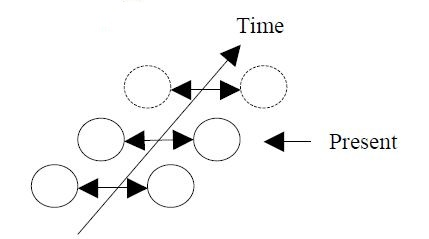
\includegraphics[scale=0.5]{interpersonal.jpg}
\caption{Eksisterende relasjon og avbrudd}
\label{interpersonal}
\end{figure}

\noindent
Avbrudd kan også ha effekter på andre mennesker som befinner seg på samme lokasjon som den som blir avbrutt. Dette illustreres i figur \ref{collateral}, hvor interaksjonen mellom aktør D (avbryter) og aktør B (den som avbrytes) også påvirker aktører A og C.
\begin{figure}[H]
\centering
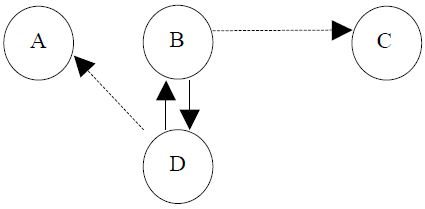
\includegraphics[scale=0.5]{collateral.jpg}
\caption{Lokasjonsbasert forstyrrelse}
\label{collateral}
\end{figure}

\noindent
En annen situasjon som kan oppstå er det Harr og Kaptelinin (2007) kaller frysing. Dersom aktører B og C utfører en oppgave ved synkron kommunikasjon, eksempelvis ansikt-til-ansikt eller per telefon, og aktør A avbryter aktør B, vil aktør C måtte vente til aktør B igjen blir tilgjengelig. 
\begin{figure}[H]
\centering
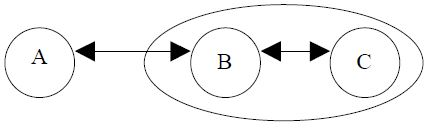
\includegraphics[scale=0.5]{frysing.jpg}
\caption{Frysing}
\label{frysing}
\end{figure}

\noindent
For en gruppe samarbeidende individer, vil oppgaver utført av et enkelt individ ofte være deler av den overordnete kollektive aktiviteten. Dermed vil forstyrrelsen av et individ sannsynligvis påvirke andre medlemmer i gruppen. Figur \ref{direkte} viser aktør B og aktør C som samarbeider om en gruppeoppgave GT, hvor GT er en del av den overordnete aktiviteten CA. Dersom aktør A avbryter aktør B, vil aktør C kanskje måtte dekke for aktør B, frem til B igjen blir tilgjengelig.
\begin{figure}[H]
\centering
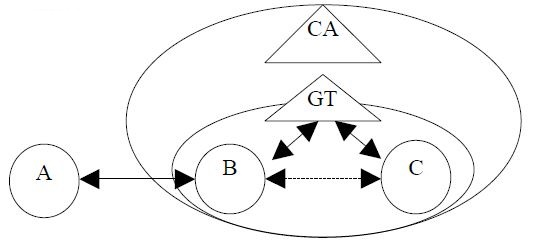
\includegraphics[scale=0.5]{coverme.jpg}
\caption{Samarbeid og avbrudd - direkte forstyrrelse}
\label{direkte}
\end{figure}

\noindent
Aktører B og C må ikke nødvendigvis kommunisere direkte, men aktør C kan være avhengig av tiden, innholdet og kvaliteten aktør Bs oppgave resulterer i. Dermed kan en forstyrrelse av aktør B også indirekte forstyrre aktør C.
\begin{figure}[H]
\centering
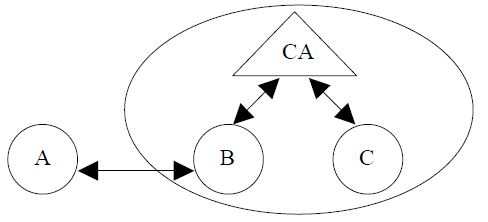
\includegraphics[scale=0.5]{dropball.jpg}
\caption{Samarbeid og avbrudd - indirekte forstyrrelse}
\label{indirekte}
\end{figure}

\noindent
Forskere som arbeider innen \emph{interruption value evaluation}-paradigmet tar utgangspunkt i at ikke alle avbrudd er dårlige, og at de ikke bør evalueres kun avhengig av hvordan de påvirker lokal kontekst, men også avhengig av hvor stor nytte de har. Målet er dermed å optimalisere individets beslutningstakingsprosess om hvordan han skal respondere på avbruddet. Den mest aktuelle teknikken for avbruddshåndtering vil derfor være forhåndsvisning av informasjon om avbruddet, hvem det er fra og hva det handler om, slik at individet selv kan reflektere over hvordan han/hun skal respondere basert på sin lokale kontekst. Dermed vil også det Grandhi og Jones (2010) kaller relasjonell kontekst være en del av avbruddskonteksten. Denne defineres som alle aspekter mellom den som avbryter og den som blir avbrutt, hvilken relasjon de har, hva avbruddet dreier seg om og deres tidligere interaksjonsmønstre.

\subsubsection{Utfordringer}
Harr og Kaptelinin (2007) påpeker tre fundamentale utfordringer ved avbruddshåndtering: (1) fare for å miste informasjon, (2) mindre privatliv og (3) utsettelse av oppgaver. For hver situasjon må individer finne den optimale balansen mellom isolasjon og tilgjengelighet, åpenhet og privatliv, og direkte eller utsatt håndtering av avbruddene.
\begingroup
\let\clearpage\relax
\section{Suksesskriterier ved implementering}
\label{chp: suksesskriterier}


\subsection{Brukbarhet}
\label{chp: brukbarhet}

Brukbarhet defineres i ISO 9241-11 \cite{Svanes08} som

\noindent
\begin{otherlanguage}{english}
\emph{the extent to which a product can be used by specified users to achieve specified goals with effectiveness, efficiency and satisfaction in a specified context of use.}
\end{otherlanguage}

\noindent
Brukbarhet er dermed et begrep som ikke kan måles generelt, men er relativt til bestemte brukere med bestemte mål i en spesifikk kontekst. Likevel kan man generelt definere noe som brukbart dersom det er funksjonelt, effektivt og tilfredsstillende \cite{Kuniavsky}. Et system er funksjonelt når det anses som nyttig av brukeren, og må dermed svare til de forventningene brukeren har til hva det skal gjøre, og faktisk gjøre det. Effektivitet kan måles som hvor raskt en er i stand til å utføre en oppgave med så lite feil som mulig. Det er vanskelig å konkretisere hva som gjør et system tilfredsstillende for en bruker, dette er individuelt og er en følelsesmessig respons ved bruk systemet \cite{Kuniavsky}. Ofte vil god design være avgjørende for om en bruker opplever systemet på en god måte, forutsett at det også er funksjonelt og effektivt. Designere av grensesnitt har gjennom årene kommet frem til en rekke reningslinjer for god design. Desverre er disse ofte blitt kritisert for å være både for spesifikke og ufullstendige \cite{mmi}. 
Interaktive applikasjoner og systemer vil spesielt hemmes av dårlig design dersom de allerede er vanskelige å lære og kompliserte å bruke. Slike systemer kan også føre til katastrofale utfall dersom kritisk informasjon ikke blir presentert på en effektiv måte. Det er derfor avgjørende å ha forståelse for hva slags informasjon brukeren trenger og hvordan denne skal presenteres \cite{Ebright10}. 

\subsubsection{Gestaltprinsippene}
Gestaltprinsippene har sitt navn fra det tyske \emph{gestalten}, som betyr "å forme". Prinsippene blir ofte referert til som lover, og det finnes mange varianter utviklet av forskjellige psykologer. Det de har til felles at de forklarer hvordan vi organiserer og tolker visuelle intrykk i områder og strukturer. Disse prinsippene beskriver blant annet virkningen av plassering av fokuspunkt, organisering av elementer, fargevalg, harmoni og enkelhet, og understeker at vi alle tolker visuelle inntrykk ut ifra egne erfaringer. 
Disse prinsippene ble i utgangspunktet brukt til å foreslå hvordan statiske visuelle elementer burde presenteres. I dag er det vanlig å ta hensyn til disse retningslinjene i design av blant annet skjermbilder \cite{Chang02}. 

\subsubsection{Affordance, konseptuelle modeller og begrensninger}
Vår forståelse av hvordan vi skal bruke en gjenstand første gang vi ser den beror på tre dimensjoner: konseptuell modell, begrensninger og \emph{affordance}. Ordet affordance ble innført av psykologen J. J. Gibson. Det finnes ingen norsk oversettelse, men begrepet refererer til hva slags handling en gjenstand signaliserer når du ser den for første gang \cite{Norman99}.

\noindent
Det skilles mellom ekte affordance og oppfattet affordance, hvor det først og fremst er oppfattet affordance vi kan kontrollere i skjermdesign. Ekte affordance vil med tanke på datamaskiner være tastatur, skjerm, knapper og musepeker som signaliserer handlinger som berøring, peking, trykking og å se på. Ekte affordance finnes alstå uavhengig av hva som vises på skjermen. Det som vises på skjermen er visuelle tilbakemeldinger som viser hva vi kan gjøre, altså oppfattet affordance \cite{Norman99}.

\noindent
Affordance blir ofte forvekslet med begrensninger og konvensjoner. Vi kan si å ha tre typer begrensninger:
\begin{enumerate}
\item Fysiske begrensninger, som har sammenheng med ekte affordance. Et eksempel på dette kan være at det er ikke mulig å flytte musepekeren utenfor skjermen. 
\item Logiske begrensninger er sterkt knyttet til en god konseptuell modell. Et eksempel på dette er hvordan brukeren vet at den må skrolle for å se resten av siden.
\item Kulturelle begrensninger er tillært og deles av en gruppe mennesker, eksempelvis hva det betyr når markøren skifter form.
\end{enumerate}
En konvensjon er en kulturell begrensning som har utviklet seg over tid, og som forbyr noe og oppfordrer til noe annet. Slike konvensjoner er langsomme, i den betydning at det tar lang tid før de blir adoptert, og når de først er blitt det, tar det vel så lang tid før de forsvinner \cite{Norman99}.

\noindent
Spesielt logiske og kulturelle begrensninger er sterke virkemidler innen skjermdesign, da designere er mer opptatt av hva brukerene oppfatter som mulig, fremfor hva som faktisk er sant. Tilbakemeldinger og reaksjoner fra skjermen hjelper oss å forstå hva vi kan og skal gjøre \cite{Norman99}.
\endgroup
\subsection{Utfordringer med CSCW}
\label{chp: utfordringerMedCSCW}

Mange CSCW-systemer faller til kort når det kommer til forventningene til deres suksess. Dette kommer gjerne til syne ved at de tiltenkte brukerene ganske enkelt unngår å bruke systemet, eller at de stadig må lage midlertidige løsninger (workarounds) for å få gejnnomført arbeidsoppgavene sine. Spesielt to grunner til dette er knyttet til kompleksiteten rundt å utvikle multibrukersystemer, som brukes samtidig av mange brukere på forskjellige nivåer og med forskjellige behov og perspektiver.

\noindent
For det første er det ofte manglede kunnskap om CSCW (multibruker-)systemer, i motsetning til enkeltbruker-systemer. En typisk CSCW-applikasjon eller system vil vanligvis bli brukt av et vidt spekter av forskjellige brukere, med forskjellig bakgrunn, erfaringer og forhold til bruk av informasjonssystemer generelt. Beslutningstakere, ofte ledere, vil ha en intuisjon for hva som vil være fordelaktige for brukere som en selv. Desverre kan de fort overse funksjoner som andre brukere vil ha nytte av, spesielt for fuksjoner som vil før til merarbeid for dem selv. 

\noindent
Det andre er at det vanskelig å lære fra tidligere feil, da CSCW-systemer er svært komplekse og unike for hvert enkelt tilfelle, noe som vanskeliggjør evaluering i ettertid. Det er også vanskelig, om ikke umulig å gjenskape miljøene og forholdene som er essensielle i den virekelige konteksten hvor et CSCW-system skal implementeres i et laboratorium. for ikke å snakke om utfordringene ved å gjøre feltobservasjoner, grunnet blandt annet variasjon i gruppesammensettning og miljømessige faktorer.


\subsection{Workarounds}
\label{chp: workarounds}

Workarounds defineres av Kobayashi (2005) som \emph{"informal temporary practices for handling exceptions to normal workflow"}. Direkte oversatt til norsk betyr det "å jobbe rundt", eller å finne midlertidige løsninger.
\noindent
Workarounds kan være nødvendig når det oppstår akutte situasjoner hvor man ikke har nødvendige ressurser tilgjengelig, eller de kan oppstå som følge av sperrer i et system. Disse sperrene kan være tilsiktede, eller utilsiktede. Et eksempel på førstnevnte finner vi i \cite{Vogelsmeier08}, hvor sykepleiere ikke kan bestille doser av medisiner høyere enn det som er anbefalt. I tilfeller hvor høyere doser likevel var skrevet ut av lege, bestilte pleierene bare flere doser. 
Et annet eksempel på en workaround er gitt av Klemets, Evjemo og Kristiansen (2013), som beskriver hvordan sykepleiere fordeler ansvar for pasienter når de skal gå til lunsj. I utgangspunktet fordeles ansvar for pasienter gjennom en bemanningsplan som konfigureres i en applikasjon kjørende på en PC i sengeområdet. Å endre på denne planen krever merarbeid, og noen sykepleiere velger derfor å ikke gjøre endringene, men heller gi muntlig beskjed til kolleger om at en går til lunsj. Dette fører til at telefonene ringer under lunsjpausen.

\noindent
Vogelsmeier (2008) beskriver workarounds som førstegrads problemløsing i den forstand at man lager mekanismer for å jobbe rundt problemer, uten å forsøke å løse den underliggende årsaken til at problemet oppsto.
Dersom workarounds oppstår som konsekvens av utilsiktede sperrer, eller der systemet er for rigid i forhold til sykepleierenes arbeidsmønster slik at systemet ikke støtter opp om arbeidet på en tilfredstillende måte, er dette svært uheldig. Dette kan i verste fall føre til livstruende situasjoner.
Selv om slike workarounds er vanlige i medisinske settinger, er de som beskrevet ikke nødvendigvis effektive og vellykkede. Workarounds som gir organisatoriske løsninger for unntak som stadig gjentar seg, og dermed reduserer den kognitive innsatsen som kreves for å håndtere nye krisesituasjoner, vil ofte være suksessfulle. Workarounds som derimot gir ringvirkninger av ustabilitet i resten av organisasjonen, kan sies å være lite suksessfulle, selv om de løser problemet der og da \cite{Kobayashi05}.
\subsection{Motstand mot endring}
\label{chp: motstand}

Implementering av nye informasjonssystemer kan by på utfordringer for ledelsen og utviklere dersom de ansatte viser motstand mot endringen. 
En slik endring vil påvirke menneskene som jobber der, deres sosiale relasjoner og forholdet mellom mennesker i og utenfor organisasjonen. Derfor kan det oppstå motstand uavhengig av hvor godt systemet som implementeres er, og i hvor stor grad de ansatte har fått bidra i utviklingen i form av medvirkning \cite{Jacobsen12}. Cavaye (1995) kaller denne motstanden for mellomliggende variabler, og understreker at sli
orhold til designer/utvikler og deres innspill blir hørt. Det finnes flere årsaker til slik motstand mot endring, og vi vil her forklare noen av dem. 

\subsubsection{Faglig uenighet}
De ansatte kan være faglig uenige i selve endringen. Verken analyser av dagens situasjon, behovet for endring eller selve endringen er klare og objektive størrelser, og det er derfor også rom for uenigheter rundt det faktiske behovet for endring, og hvorvidt endringen som gjennomføres er den rette løsningen på problemet. \cite{Jacobsen12}

\subsubsection{Merarbeid}
En endring i seg selv kan kreve ekstraarbeid fra de ansatte, spesielt i en overgangsfase. Det kan være mye nytt å sette seg inn i og lære, noe som krever en ekstra innsats, ofte uten tilstrekkelig kompensasjon, noe mange stiller seg negative til. Slikt ekstraarbeid kan i tillegg til å lære noe nytt innebære at man må avlære de gamle måtene å jobbe på. \cite{Jacobsen12}

\subsubsection{Systemet som en trussel}
Dersom brukerene ser på det nye systemet som en trussel mot deres nåværende kontroll over eget arbeid, eller deres posisjon i form av deres ekspertise, vil de mest sannsynlig motsette seg endringen det nye systement representerer. \cite{Cavaye95}

\subsubsection{Grad av medvirkning}
Motstand kan også oppstå dersom det faktiske nivået av medvirkning avviker fra det nivået brukeren ønsker seg. Dette gjelder ikke bare dersom nivået er lavere, men også dersom nivået av medvirkning blir høyere enn det brukeren så for seg i utgangspunktet. Det er derfor ikke tilstrekkelig med medvirkning i seg selv, den må også møte brukerenes forventninger. \cite{Cavaye95}

\noindent
Jacobsen(2012) hevder at indre motivasjon og involvering de ansatte, slik at de føler seg som medeiere i endringsprosessen er avgjørende for å få de ansatte motivert for endringen og dermed redusere overnevnte motstand. Bred deltagelse på denne måten gir den enkelte ansatte opplevelsen av at den er med på å forme sin egen fremtid, og at dette vil skape en aksept og forståelse for usikkerheten som er assosiert med en hver endring.
\subsection{Brukermedvirkning og deltagende design}
\label{chp: medvirkning}

\subsubsection{Brukermedvirkning}
Uttrykket \emph{brukermedvirkning} er sammensatt av to aspekter, \emph{bruker} og \emph{medvirkning}. For å forstå hva brukermedvirkning egentlig er må vi forstå de to aspektene enkeltvis. Vi må anerkjenne at det finnes flere typer \emph{brukere}. Det kan være toppledelsen, som bruker systemets output i sine analyser og strategiske avgjørelser. Det kan være mellomledere som er ansvarlig for, og overvåker, avdelinger som bruker systemet. Til sist har vi de ansatte som bruker systemet i sitt daglige arbeid. Det er ofte naturlig at alle brukergruppene tar del i utviklingsprosessen i større eller mindre grad. Toppledelsen må kanskje godkjenne systemet, og kan ha meninger om hva slags rapporter det skal generere. Mellomledelsen og andre ansatte kan bidra med innsikt i dagens arbeidsrutiner, problemer og workarounds, samt kravspesifikasjoner, ønsker til design og testing. Vi må også forstå at \emph{medvirkning} ikke er det samme som involvering, selv om de to uttrykkene ofte blir brukt om hverandre. I Cavaye (1995) finner vi definisjonene av (bruker)medvirkning og involvering som henholdsvis \emph{"a set of operations and activities performed by users"} i løpet av utviklingsprosessen, og \emph{"subjective psycological state"} som påvirker brukernes forestillinger, og dermed systemets grad av suksess.

\noindent
Brukermedvirkning finner vi i mange former og på flere nivåer. Som vi ser i tabell \ref{Beskrivelse av brukermedvirkning} kan medvirkning beskrives ved hjelp av flere attributter. 

\begin{table}[H]
\caption{Beskrivelse av brukermedvikrning (hentet fra Cavaye (1995))}
%\centering
\begin{tabular}{c c}
\hline\hline
\textbf{Medvirkningsattributter} & \textbf{Mulige verdier} \\ [2ex]
\hline
& alle brukere \\[-1ex]
\raisebox{1.5ex}{Type} & representativt utvalg av brukere \\ [2ex]
\hline
& rådgivende \\ & signeringsansvar  \\
\raisebox{2ex}{Grad} & del av teamet \\ & fullt ansvar \\ [2ex]
\hline
& teknisk design \\
\raisebox{1.5ex}{Innhold} & sosialt og teknisk design \\ [2ex]
\hline
& prosjektdefinering  \\ & kravspesifikasjon  \\
\raisebox{2ex}{Område} & utvikling \\ & testing \\ [2ex]
\hline
& formell \\
\raisebox{1.5ex}{Formalitet} & uformell \\ [2ex]
\hline
& innspill ignorert \\
\raisebox{2ex}{Innflytelse} & bidrag tatt i betraktning  \\ & innspill tas seriøst \\
\hline
\end{tabular}
\label{Beskrivelse av brukermedvirkning}
\end{table}

\begin{itemize}
\item Type medvirkning beskriver andelen av brukere som faktisk blir inkudert. Det er ikke alltid det lar seg gjøre å inkludere alle brukere i praksis. Da er det viktig å etterstrebe å ha et representativt utvalg av disse med i prosessen.
\item Grad av medvirkning viser til at brukere har forskjellig grad av ansvar gjennon sin medvirkning.
\item Innholdet i medvirkningen refererer til det faktum at brukerne kan involveres i forskjellige aspekter av utviklingsprosessen. Det er vanlig at brukere involveres i aktiviteter som forbereder det tekniske designet av systemet, men de kan også involveres i det sosiale designet, det vil si de menneskelige og sosiale effektene systemet vil ha.
\item Området medvirkningen angår vil variere gjennom de forskjellige fasene av utviklingsprosessen. Medvirkning fra brukerne er mer vanlig i forbindelse med å sette rammer for prosjektet, kravsspesifikasjon og testing enn gjennom selve utviklingen og kodingen av systemet.
\item Medvirkningen kan være formell, ved bruk av formelle grupper og team, eller uformell, med tilfeldige diskusjoner og oppgaver.
\item Innflytelsen brukerene faktisk har kan variere, og innspill fra disse kan vektlegges i forskjellig grad av utviklerene, alt fra å bli totalt ignorert til å bli tatt svært seriøst. Dette betyr at det kan legges ned mye ressurser i å la brukerne få komme med innspill, men at virkningen av disse beror på i hvilken grad disse blir tatt hensyn til.
\end{itemize}

\noindent
I mange år ble det sett som en selvfølge at brukermedvirkning hadde en signinfikant positiv effekt på en eventuell suksess for et informsjonsystem. Empiriske studier kan imidlertid ikke bevise at det alltid er en slik sammenheng \cite{Cavaye95}. Dermed ser det ut til at brukermedvirkning hverken er tilstrekkelig eller ytterst nødvendig for å garantere suksess for et informasjonsystem. 
Det er flere grunner til dette, sett fra både designers/utviklers og brukerens side. For det første har forholdet mellom bruker og designer/utvikler stor innvirkning på effekten av medvirkningen. Forskjeller i bakgrunn, erfaring og perspektiver kan føre til konflikter som igjen preger effekten av medvirkningen på en negativ måte. For det andre spiller det ingen rolle i hvor stor grad brukerne medvirker i prosessen dersom deres innspill blir ignorert. For det tredje vil de ansattes motstand mot endring kunne resultere i ubrukte systemer, eller bevisst sabotasje av implementeringen og endringsprosessen. Som beskrevet i avsnitt \ref{chp: motstand}, vil motstand mot endring kunne reduseres ved god informasjon og involvering (til forskjell fra medvirkning) av de ansatte. Dette må ikke sees som en motsetning til Cavaye (1995)s påstand om at medvirkning ikke er en garanti for suksess. Dette fordi informasjon til og involvering av de ansatte ikke nødvendigvis behøver å inkludere medvirkning, og fordi selv med medvirkning og innspill fra de ansatte er en ikke garantert å redusere motstanden tilstrekkelig til å sikre en suksessfull implementering av det nye systemet \cite{Cavaye95}.

\subsubsection{Deltagende design}
\label{dd}
Deltagende design er én av mange teknikker for å oppnå brukermedvikning.
Interessen for denne teknikken blir stadig større, og sees på som en god måte å blant annet sikre gode innspill fra brukere (for blant annet analyse av dagens situasjon), gjensidig læring og bedring av arbeidsrutiner.

\noindent
Vi kan dele utvikling av informasjonsystemer i tre aspekter: analyse, design og praksis. Det kan være vanskelig å kombinere alle tre samtidig, og tidligere ble det sett på som svært positivt om man greide å kombinere to av disse. Mogensen og Trigg (1992) ser i sin studie på muligheten for å kombinere alle tre aspektene samtidig (figur \ref{Challenge_PD}).

\begin{figure}[H]
\centering
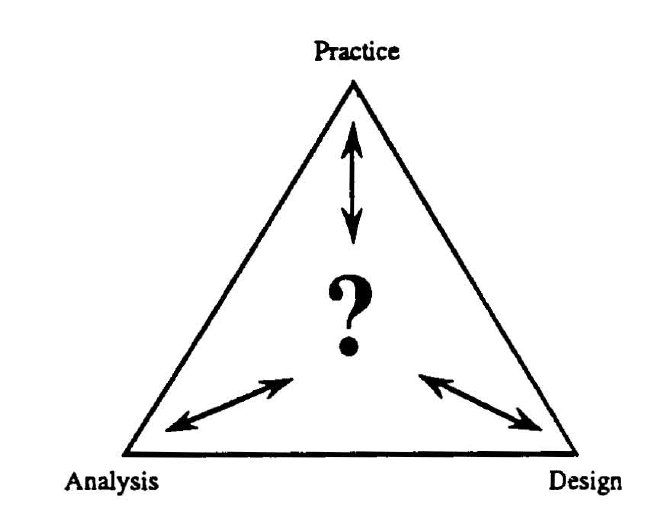
\includegraphics[scale=0.3]{Challenge_PD.jpg}
\caption{Hvordan kombinere alle?}
\label{Challenge_PD}
\end{figure}

\noindent
Ifølge \cite{Mogensen92} er det flere måter å oppnå større medvirkning på. Én teknikk er \emph{fremtidsworkshops}, der en ønsker diskusjon rundt mulige fremtidige løsninger på nåværende problemer, identifisert av brukerne selv. En annen teknikk er workshops hvor en bruker mock-ups og prototyper for å trigge diskusjon om mulige fremtidige teknologier og løsninger. Uavhengig av valgt teknikk vil graden av relevans til dagens praksis være avgjørende for workshopens suksess. Felles for de to er at de tar i bruk kontekstuelle artefakter (artefakter medbrakt av fasilitator som brukerene selv setter i kontekst).

\noindent
Mogensen og Trigg (1992) konkluderer med at bruk av kontekstuelle artefakter og hvor alle de tre faktorene, analyse, praksis og design er tilstede kan lede til nettopp et slikt ønsket samspill som vist i figur \ref{Artifacts_PD}. De argumenterer for at bruk av artefakter under en workshop ikke bare gir innspill på design - deltagende design, men at de også kan trigge diskusjoner som gir utviklerene bedre innsyn i dagens praksis, problemer og workarounds - deltagende analyse. 

\noindent
Deltagende design på denne måten, med bruk av kontekstuelle artefakter, gir derfor forskere/utviklere en dypere forståelse av hva som er problemområdene, og hvordan brukerne selv oppfatter dagens situasjon. Det gir også brukerne mulighet til større bevissthet rundt egne arbeidsmetoder, -rutiner og workarounds.

\begin{figure}[H]
\centering
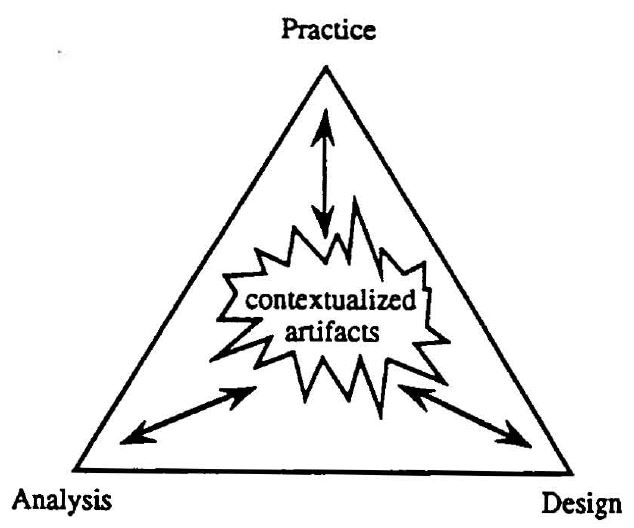
\includegraphics[scale=0.3]{Artifacts_PD.jpg}
\caption{Kontekstuelle artefakter støtter samspillet mellom de tre perspektivene}
\label{Artifacts_PD}
\end{figure}
\subsection{Suksesskriterier for implementering av informasjonsystemer ved sykehus}
\label{chp: suksess_sykehus}

Vi har i dette kapittelet sett på noen av elementene som kan påvirket graden av suksess ved implementering av nye informasjonsystemer. Mange av dem, som brukbarhet og motstand [EDIT ETTER BEHOV], er generelle for utvikling og implementering og vil ikke bli gått nermere inn på i denne delen. Vi vil heller trekke frem spesielle hensyn som er viktige å ta når man utvikler og implementerer informasjonsystemer spesielt for sykehus og det spesielt komplekse systemet dette er.



\noindent
Slike strømlinjeformede og rasjonaliserte informasjonsystemer vil også føre til et stort behov for workarounds, nettopp fordi det hele tiden vil oppstå situasjoner hvor det ikke er ønskelig, eller mulig å gjennomføre en oppgave slik informsjonsystemet tilsier at det skal gjøres. 

\noindent
Vi ser gjennom dette at informasjonsystemer utviklet for bruk på sykehus må ha en svæt stor åpenhet, og så liten grad av fastsatte rutiner og sekvenser som mulig.
\chapter{Forskningsmetode og hensikt}
\label{chp:forskningsmetode}

“I just want to develop a computer-based system” (Oates, 2006)

\noindent
Ifølge Oates (2006) er design og utvikling av ethvert databasert produkt en form for forskning som krever innsamling av data, analyse og konklusjon. For å utvikle et produkt eller system som skal utføre gitte oppgaver er det viktig å besvare hva disse oppgavene er, og hvorfor de er viktige. Dette besvares ved å samle informasjon om hva man ønsker av systemet, generere egen data som dokumenterer hvordan og hvorfor man designer og implementerer produktet, og deretter brukerteste og evaluere det. Vi vil i dette kapittelet først presentere hensikten med prosjektet før vi går i detalj på hvilke tilnærminger og metoder vi har valgt for å besvare forskningsspørsmålene.


\section{Hensikt}
\label{chp: hensikt}

Hensikten gjenspeiler den underliggende grunnen til å gjøre forskning, hva som gjør den interessant og hvorfor den er viktig eller nyttig. Videre kan man se på hvorfor man ønsker å forske på noe \cite{Oates}. 

\noindent
Motivasjonen for oppgaven var innledningsvis å avdekke fordeler og utfordringer i det eksisterende pasientsignalsystemet, og hvordan det kunne videreutvikles for å bedre støtte sykepleierenes behov. En gjennomgang av tidligere arbeid ga en bredere forståelse av forskningsområdet, og vi ønsket derfor å utdype problemstillingen. Vi formulerte to forskningsspørsmål som søkte svar på hvorvidt informasjon om kollegers aktiviteter og tilgjengelighet er nyttig, og hvordan slik informasjon kan kommuniseres på en hensiktsmessig måte. Da tidligere arbeid viste at avbrytelser kan ha en negativ effekt på sykepleieres arbeid, ønsket vi samtidig å undersøke hvordan systemet kan endres for å redusere eventuelle negative effekter.

\subsubsection{Forskningsspørsmål}
Vi har formulert to spørsmål som vi søker svar på gjennom denne oppgaven. Disse er som følger:

\begin{enumerate}
\item Er informasjon om kollegers aktiviteter og tilgjengelighet nyttig for sykepleiere, og hvordan kan slik informasjon distribueres på en hensiktsmessig måte? 
\item Hvordan kan systemet endres for å begrense potensielle negative effekter ved avbrytelser?
\end{enumerate}

\section{Prosess}
\label{chp: prosess}

Prosessen i et forskningsprosjekt kan beskrives som sekvensen av aktiviteter som utføres i løpet av prosjektets varighet \cite{Oates}. Vi vil nå gjøre rede for de metodene og tilnærmingene vi har valgt i vår prosess.

\subsection{Paradigme}
Et paradigme er et sett felles antakelser om, eller måter å tenke på, noen aspekter av verden \cite{Oates}. Innen samfunnsforskningen fremstår kvalitativ og kvantitativ forskning som to vesentlige tenkemåter, eller paradigmer, når det gjelder hvordan man kan framskaffe eller generere informasjon om samfunnet, for deretter å analysere det (Tjora, 2010).
[SKRIV OM KVALITATIV vs KVANTITATIV, INDUKTIV, DEDUKTIV OG ABDUKTIV]

\subsection{Litteraturstudie}
Teorien vi har lagt frem i kapittel \ref{chp:teori} er basert på et litteraturstudie gjort innledningsvis i arbeidet. For å definere forskningsspørsmålene knyttet til oppgaven, analyserte vi i første omgang tidligere arbeid gjort av Klemets, Evjemo og Kristiansen (2013). Dette ga oss et inntrykk av forskningsområdet og utfordringene knyttet til det eksisterende pasientsignalsystemet. 

\subsection{Dokumentstudie}

\subsection{Prototype}
Ifølge Schneiderman og Plaisant (2010) mislykkes mange utviklingsprosjekter i å nå sine mål, i stor grad grunnet dårlig kommunikasjon mellom utviklere og brukere. Suksessfulle utviklere legger derfor stor vekt på å forstå kundens behov og krav. 
Brukersentrert design gir systemer som genererer færre problemer under utviklingen, og lavere vedlikeholdskostnader. De er enklere å lære, gir raskere ytelse og vesentlig mindre feil \cite{mmi}.
Prototyping er en velkjent måte å utforske og uttrykke design for interaktive systemer. 

\tikzstyle{mybox} = [draw=black, fill=white, very thick,
    rectangle, inner sep=10pt, inner ysep=20pt, rounded corners]
\tikzstyle{fancytitle} =[fill=black, text=white]
\begin{tikzpicture}
\node [mybox] (box){%
    \begin{minipage}{0.9\textwidth}
      En prototype defineres som enhver representasjon av en designidé, uavhengig av medium \cite{Houde97}.
    \end{minipage}
};
\node[fancytitle, rounded corners, right=10pt] at (box.north west) {Definisjon av prototype};
\end{tikzpicture}%



\chapter{Resultater}
\label{chp:resultater}

Resultatene i denne oppgaven kan deles i to deler. Den første er prototypen, som er et resultat av den innledende gjennomgangen av teori, som ga grunnlaget for valg av funksjonalitet. Den andre delen av resultatene er funn gjort under workshopene. Disse ga utfyllende kunnskap om hvordan sykepleierstudentene jobber i dag, og hvordan de håndterer ulike situasjoner ved innkommende pasientsignaler. Vi fikk innspill på hva de opplevde som fordeler og utfordringer ved det eksisterende systemet, og deres syn på vår foreslåtte løsning. 
\section{Prototypen}
\label{prototypen}

Vår prototype, som er et resultat av omfattende kvalitative litteraturstudier, er basert på bruk av smarttelefoner, i motsettning til telefonene fra cisco som er i bruk i dag. Grunnen til dette valget ligger i at dette er mer fremtidsrettet og gir bedre mulighet for mer utfyllende informasjon i skjermbildet, samtidig som det også gir mulighet for interaksjon med brukeren og åpner for å senere legge til funksjunalitet som eksempelvis å hente frem annen informasjon, som journaler og prøvesvar. Vi har etterstebet å lage et intuitivt design, som gir god informasjon for å støtte awareness.

\noindent
Applikasjonen er tenkt å være den eneste kjørende på telefonen, hvor vanlige funksjoner som telefon er inkludert, slik at det kun er denne applikasjonen som brukes - også for vanlige telefonsamtaler. Vi vil i de neste delene gi en forklaring på prtotypens design og funksjonalitet. Da dagens pasientsignal-system er beskrevet i appendiks \ref{appendix_dagenssystem} vil vi oppfordre leserene til å lese dette appendikset ved uklarheter rundt systemets oppbyggning og funksjonalitet.

\noindent
En antagelse som er gjort er at det er implementert systemer for lokalisering av sykepleierene, slik at systemet kan vite hvilket rom sykepleierene er i til en hver tid. Denne funksjonen vil bli brukt av statusindikatoren beskrevet senere i dette kapittelet. Bardram (2004) trekker frem at mange sykepleiere er skeptiske til slik sporing, med begrunnelse i at det i ettertid kan lages statistikker på hvor lenge man er hvor, som blandt annet på pauserommet. Vårt forslag er å ikke lagre denne informasjonen i det hele tatt, slik at den heller ikke kan brukes mot sykepleierene i ettertid. I forhold til systemet har informsjonen kun verdi i sanntid, og det er derfor ingen grunn til å lagre denne informsjonen.

\noindent
Presentasjon av pasientsignalet, formidling av sykepleierenes tilgjengelighet og spesielt kombinasjonen av disse har vært vårt hovedfokus i utviklingen av denne prototypen. Det er derfor også disse som er lagt mest vekt på i dette kapittelet. De øvrige fonksjonene og skjermbildene er med for å skape et helhetlig inntrykk av prototypen, og for å hjelpe deltagerene på workshoppene til å se muligheter og komme på egne ideer til hva de mener vil være nyttig funksjonalitet og informasjon.

\subsection{Tilgjengelighet og pasientsignal}
Disse to er tett knyttet sammen for å assistere sykepleierene i valget om de skal godta eller avvise et pasientsignal. Kunnskap om kollegers tilgjengelighet kan også legges til grunn ved avgjørelser angående om, og hvordan, man skal ta kontakt med andre sykepleiere. Teorien som er lagt til grunn for valgene vi har gjort her er presentert i \ref{chp: kognisjon}, \ref{chp: awareness} og \ref{chp: avbrudd}.

\subsubsection{Tilgjengelighet}
Tilgjengelighet-indikatoren har som formål å fortelle sykepleieren om hvilken tilgjengelighet han/hun er satt som for øyeblikket. Vi har valgt å bruke tre forskjellige statuser; "tilgjengelig"\ (grønn), "på rom"\ (gul), og "opptatt"\ (rød) (figur \ref{tilgjengelighetsstatuser}). Denne er i utgangspunktet satt som tilgjengelig. Når sykepleieren går inn på et rom vil denne automatisk skiftes til "på rom", og motsatt når sykepleieren forlater rommet og går ut på gangen/tunet igjen. Dersom sykepleieren vet at oppgaven som skal utføres vil ta lang tid, og han/hun helst ikke vil forstyrres i løpet av denne tiden, kan statusen manuelt settes til "opptatt". Dette signaliserer til de andre sykepleierene at dersom det er mulig, skal en unngå å kontakte denne sykepleieren, da det vil forårsake en uønsket forstyrrelse. Denne statusen vil bli stående til sykepleieren igjen endrer status til "tilgjengelig". Eventuelt kan det gis en påminnelse etter en fastsatt tid som spør sykepleieren om det er meningen at statusen fremdeles skal være "opptatt". Teknologien som ligger bak denne automatikken er ikke en del av denne oppgaven.

\begin{figure}
	\centering
	\begin{subfigure}[b]{0.3\textwidth}
		
\includegraphics[scale=0.15]{statusGronn.jpg}
		\caption{Tilgjengelig}
		\label{proto_startside}
	\end{subfigure}
	\begin{subfigure}[b]{0.3\textwidth}
		
\includegraphics[scale=0.15]{statusGul.jpg}
		\caption{På rom}
		\label{proto_startside}
	\end{subfigure}
	\begin{subfigure}[b]{0.3\textwidth}
		
\includegraphics[scale=0.15]{statusRod.jpg}
		\caption{Opptatt}
		\label{proto_startside_medMeny}
	\end{subfigure}
	\caption{Tilgjengelighetsstatuser}
	\label{tilgjengelighetsstatuser}
\end{figure}

\subsubsection{Pasientsignal}
Dette er en av de største endringene fra dagens system, og en av hovedfunksjonene med tanke på vår oppgave. Eksempel på enhetene som er i bruk i dag er avbildet i figur [SETT INN REF], mens skjermbilde ved pasientanrop ved bruk av prototypen er avbildet i figur \ref{protoPasientsignal}. Den største endringen vi har gjort, borstestt fra design, er at det vises en liste over de neste sykepleierene, samt deres tilgjengelighet, som vil bli oppringt dersom sykepleieren velger i avvise anropet. Hensikten med denne listen er å tilgjengeliggjøre informasjon som kan gi sykepleieren bedre grunnlag for avgjørelsen i forhold til om anropet skal godtas eller avvises.

\begin{figure}[H]
\centering
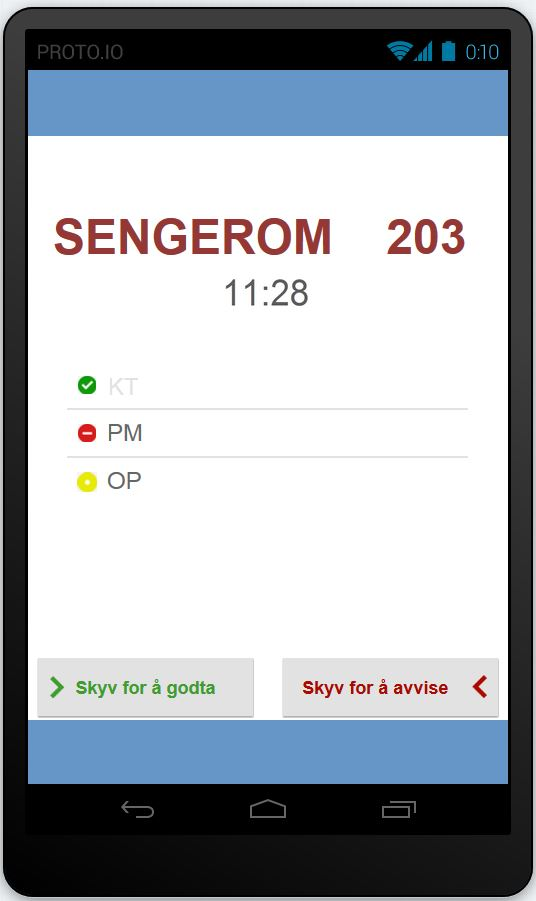
\includegraphics[scale=0.4]{proto_pasientsignal.jpg}
\caption{Skjermbilde ved inkommende pasientsignal. Her fra sengerom 203}
\label{protoPasientsignal}
\end{figure}

Med denne informsjonen umiddelbart tilgjengelig når en pasient ringer har sykepleieren mulighet til å, dersom han/hun ser at det er andre sykepleiere som er tilgjengelig, avvise anropet uten å være bekymret for at pasienten ikke får hjelp. Dette vil i andre omgang frigjøre kapasitet i arbeidsminnet (\ref{chp: kognisjon}) og dermed kan sykepleieren være mer mentalt tilstede hos pasienten som han/hun er hos på dette tidspunktet, som igjen gir bedre pasientomsorg.

\subsection{Skjermbildene og deres funksjon}

Som nevnt over er det paisentsignalet, og awareness-informsjonen som bilr kommunisert sammen med dette som er hovedfokuset i denne oppgaven. De øverige skjermbildene som her vil be presentert er laget av to grunner: de skal gi prototypen en mer helhetlig fremtoning, og de skal representere fremtidsrettet tankegang for fremtidig funksjonalitet, som kan være med å trigge kreativ tenkning hos deltagerene på workshoppene.

\subsubsection{Startsiden}
Forsiden er som ilustrert i figur \ref{proto_startside}. Knappen øverst til venstre gir tilgang til en dorp-down meny som vist i figur \ref{proto_startside_medMeny}. 

\begin{figure}[H]
	\centering
	\begin{subfigure}[b]{0.48\textwidth}
		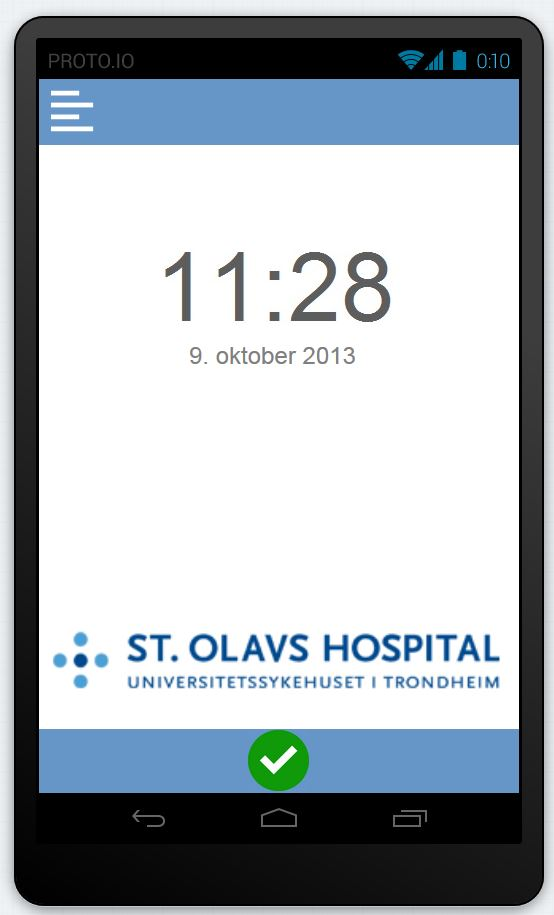
\includegraphics[scale=0.4]{proto_startside.jpg}
		\caption{Prototypens startside}
		\label{proto_startside}
	\end{subfigure}
	\begin{subfigure}[b]{0.48\textwidth}
		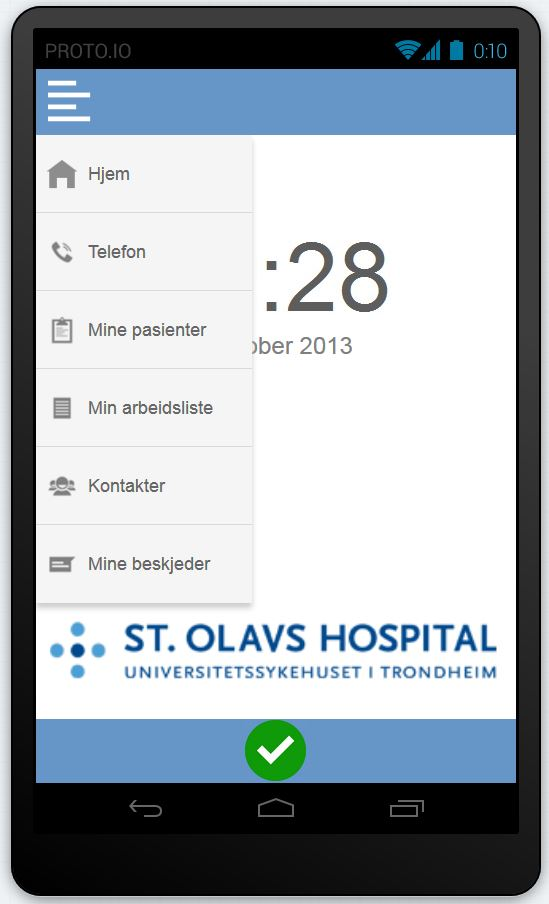
\includegraphics[scale=0.4]{proto_startside_medMeny.jpg}
		\caption{Prototypens startside med menyvisning}
		\label{proto_startside_medMeny}
	\end{subfigure}
	\caption{Prototypens startside}
\end{figure}

\noindent
Forsiden er ment som en standby-side, det vil si at det er denne siden som vises når skjermen slåes på. Tanken var at denne skal være enkel, med få elementer. Vi har derfor valgt kun klokke og datovisning i tillegg til status-indikatoren, midt på det nederste blå feltet (her illustrert med en grønn sirkel med hvit hake), og menyknappen øverst til venstre. Status-indikatoren og menyknappen vises på alle skjermbilder. 

\subsubsection{Min Arbeidsliste}
Her vises alle psientsignal du har godtatt, men ikke vært hos. Dette betyr at dersom du velger å godta et pasientsignal vil det legges i denne listen. Når du har gått inn på rommet hvor signalet ble utløst, vil elementet forsvinne fra listen. Dersom en sykepleier har godtatt flere psientsignal vil det da ligge flere elementer i listen. Dette er ment til å være til hjelp slik at sykepleieren ikke skal glemme noen av pasientene, selv om han/hun skulle bli avbrutt. Funksjonen vil på denne måten avlaste arbeidsminnet (se kapittel \ref{chp: kognisjon}) til sykepleierene slik at de kan være mer mentalt tilstede, og bedre kunne fokusere på oppgaven de holder på med.

\subsubsection{Mine Pasienter}
Dette er nok den funksjonen som er mest fremtidsrettet og åpen for mer informsjonsflyt slik prototypen står i dag. Sykepleierene fordeler pasientene mellom seg ved starten av hver vakt. Ved å registrere dette i bemanningsplanen (se appendiks \ref{appendix_dagenssystem}) vil disse legges i listen "Mine Pasienter". Her er ideen at det i fremtiden kunne være mulig å aksessere journaler, tidligere prøvesvar, samt få beskjed når nye prøvesvar er klare. Som vist i figur \ref{minePasienter}, kan nye blodprøvesvar da vasles og vises direkte på telefonen. Sykepleieren ser med én gang at det er kommet ny informasjon angående Hermansen. Ved å trykke på navnet hans ser man at varselet gjelder svar på blodprøvene, og ved å trykke på teksen "nye blodprøvesvar"\ vil svarene straks vises.

\begin{figure}[H]
\centering
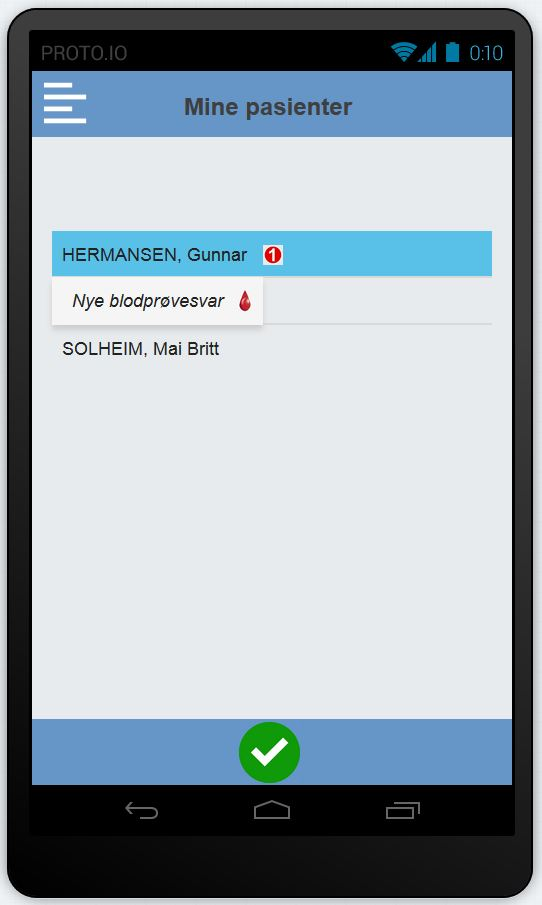
\includegraphics[scale=0.4]{minePasienter.jpg}
\caption{Eksempel på pasientlisten til en sykepleier. Her er det kommet svar på blodprøvende til Hermansen.}
\label{minePasienter}
\end{figure}

\subsubsection{Mine Beskjeder}
Mine beskjeder er en slags sms-lignende tjeneste hvor sykepleierene kan stille hverandre med spørsmål og gi beskjeder som ikke haster. Dette er en mindre forstyrrende og avbrytende måte å kommunisere på, når det ikke er avgjørende med rask respons.

\subsubsection{Kontakter}
Her vises kontaktinformasjon inkludert tilgjengelighet til de sykepleierene som er på jobb. Her skal det være enkelt å få oversikt over alle som er på vakt, og om de er tilgjengelige eller ikke. Dette er ment å brukes blandt annet dersom man har et spørsmål som flere kan svare på. Ved hjelp av kontaktlisten kan man velge den som mest sannsynlig vil bli minst forstyrret av henvendelsen. Ved å trykke på kontakten vil denne automatisk bli oppringt.

\subsubsection{Telefon}
Dette er den vanlige telefonfunksjonen vi kjenner fra vanlige telefoner, og trenger ingen detaljert forklaring.





%% include here the other chapters

\renewcommand*{\bibname}{ReferanseDatabase}
\bibliographystyle{ieeetr}
\bibliography{main}



%% Uncomment the following if you have any appendix
\appendix
\addtocontents{toc}{%
\protect\vspace{1em}% 
\protect\noindent \bfseries \appendixtocname\protect\par
  \protect\vspace{-.5em}%
 }
 \renewcommand{\chaptername}{\appendixname}
%% include below possible appendices (chapters)
\chapter{Dagens pasientsignalsystem ved St. Olavs Hospital}
\label{appendix_dagenssystem}
Dette tillegget inneholder en beskrivelse av dagens pasientsignalsystem ved St.Olavs Hospital. Tekst og bilder er hentet fra opplæringsdokumenter og brukermanualer gitt ved St. Olavs Hospital, tilgjengelig på deres hjemmesider \cite{BrukerveiledningforPasientsignal, BrukermanualforPasientsignalogPasientsignalapplikasjon, BrukerveiledningforTradlostelefon}

\section{Dagens pasientsignalsystem}
Et signal utløses fra blant annet sengerom, fellesrom, stuer og toalett, for å tilkalle/alarmere pleiepersonell. Det skilles mellom to typer signaler: (1) Pasientsignal, som utløses av pasienten selv, og (2) hasteanrop, som utløses av pleiepersonell ved behov for umiddelbar assistanse. Pasientsignalsystemet er sammensatt av to integrerte systemer, et fast og et trådløst. 

\subsection{Pasientsignalanlegget - det faste systemet}
Det faste systemet, også refererert til som pasientsignalanlegget, består av fastmonterte paneler med trekksnorer og/eller trykknapper. Disse er illustrert i figur \ref{pasientsignalanlegget}.

\begin{figure}[H]
        \centering
        \begin{subfigure}[b]{0.3\textwidth}
        		\centering
                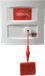
\includegraphics[scale=0.7]{anropspanel.png}
                \caption{Anropspanel}
                \label{anropspanel}
        \end{subfigure}%
        \begin{subfigure}[b]{0.3\textwidth}
        		\centering
                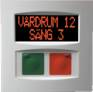
\includegraphics[scale=1.5]{rompanel.jpg}
                \caption{Rompanel}
                \label{rompanel}
        \end{subfigure}
        \begin{subfigure}[b]{0.3\textwidth}
        		\centering
                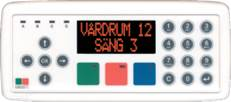
\includegraphics[scale=1]{vaktromsapparat.jpg}
                \caption{Vaktromsapparat}
                \label{vaktromsapparat}
        \end{subfigure}
        \caption{Pasientsignalanlegget}
        \label{pasientsignalanlegget}
\end{figure}

\noindent
\subsubsection{Anropspanelet}
Det finnes to typer anropspanel, et for våtrom og et for vanlig rom. I vanlige sengerom er anropspanelet plassert ved sengen, og har en trykknapp med lysdiode og en trekksnor.
Trykknappen utløser et hasteanrop, mens trekksnoren utløser et pasientsignal.

\subsubsection{Rompanelet}
Rompanelet er plassert ved døren til hvert av sengerommene på tunet. Det har et display, og en grønn og en rød trykknapp med hver sin lysdiode. Grønn knapp trykkes for å markere pleiepersonells tilstedeværelse eller for å avstille et signal. Rød knapp trykkes for å utløse pasientsignal, eller et hasteanrop dersom tilstedemarkering er aktivert. Rød knapp kan også holdes inne i 2 sekunder for å utløse hasteanrop, dersom tilstedemarkering ikke er aktivert. 

\subsubsection{Vaktromsapparatet}
Vaktromsapparatet er sentralt plassert i det åpne landskapet på sengetunet. Det består av et display og flere tall- og tegntaster. Displayet indikerer stedangivelse for et pasientsignal, hasteanrop og tilstedemarkerte rom. Pasientsignaler og hasteanrop er signalisert med rød tekst, mens tilstedemarkering er vist ved grønn tekst. Tall- og tegntastene brukes for å programmere apparatet.

\subsection{Det trådløse systemet}
Pasientsignalanlegget er videre tilkoblet det trådløse systemet, som består av følgende IKT-komponenter: pasientsignalapplikasjon, trådløs telefonenhet og pasientterminal, illustrert i figur \ref{pasientapplikasjon}, \ref{telefonenhet} og \ref{pasientterminal} henholdsvis.

\begin{figure}[H]
        \centering
        \begin{subfigure}[b]{0.35\textwidth}
        		\centering
                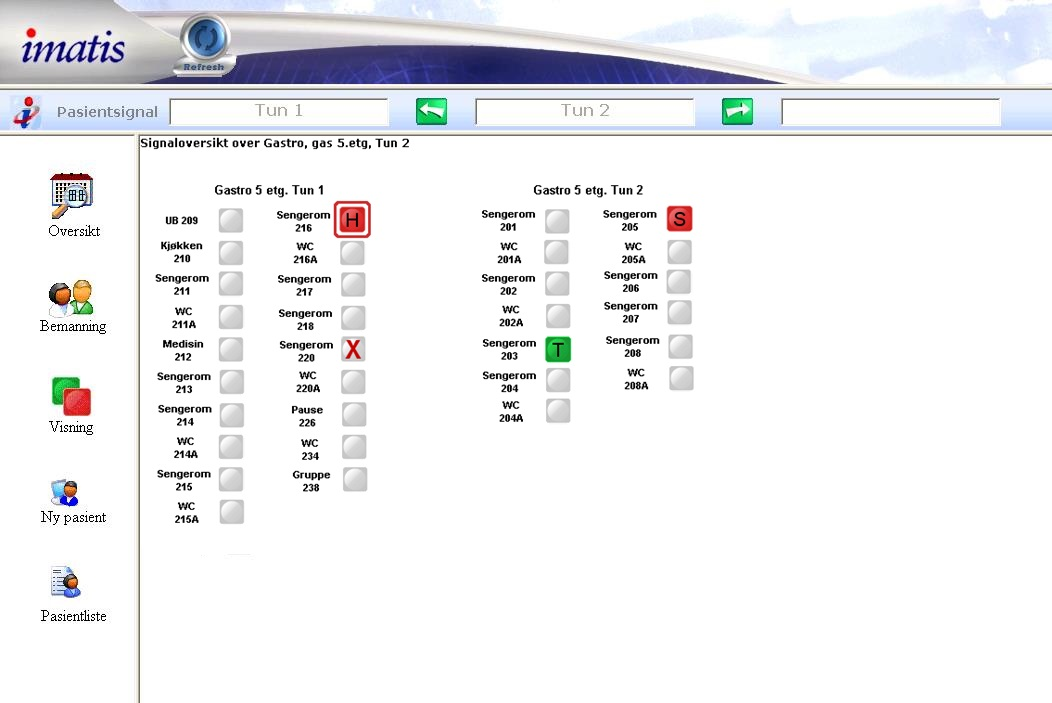
\includegraphics[scale=0.2]{pasientapplikasjon.jpg}
                \caption{Pasientsignalapplikasjon}
                \label{pasientapplikasjon}
        \end{subfigure}
        \begin{subfigure}[b]{0.35\textwidth}
        		\centering
                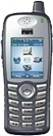
\includegraphics[scale=1]{telefon.jpg}
                \caption{Trådløs telefonenhet}
                \label{telefonenhet}
        \end{subfigure}
        \begin{subfigure}[b]{0.25\textwidth}
        		\centering
                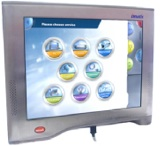
\includegraphics[scale=0.4]{pasientterminal.jpg}
                \caption{Pasientterminal}
                \label{pasientterminal}
        \end{subfigure}
        \caption{Det trådløse systemet}\label{dettradlosesystemet}
\end{figure}

\subsubsection{Pasientsignalapplikasjon}
Pasientsignalapplikasjonen kjører på en PC på hvert sengetun, 24 timer i døgnet, hver dag. Applikasjonen tilbyr i hovedsak fem funksjoner: (1) oversikt, (2) bemanning, (3) visning, (4) registrering av ny pasient og (5) en pasientliste. Vi vil her utdype funksjonene bemanning og visning, da disse er av mest relevans for vår oppgave.  

\noindent
Bemanningsplanen, vist i figur \ref{bemanningsplan}, knytter tilgjengelig pleiepersonell til rommene ved et sengetun. Pasientsignalene vil dermed sendes til riktig mottaker på bakgrunn av bemanningsplanen. For hvert rom vil det normalt tilknyttes en primærsykepleier og en disponibel sykepleier.

\begin{figure}[H]
\centering
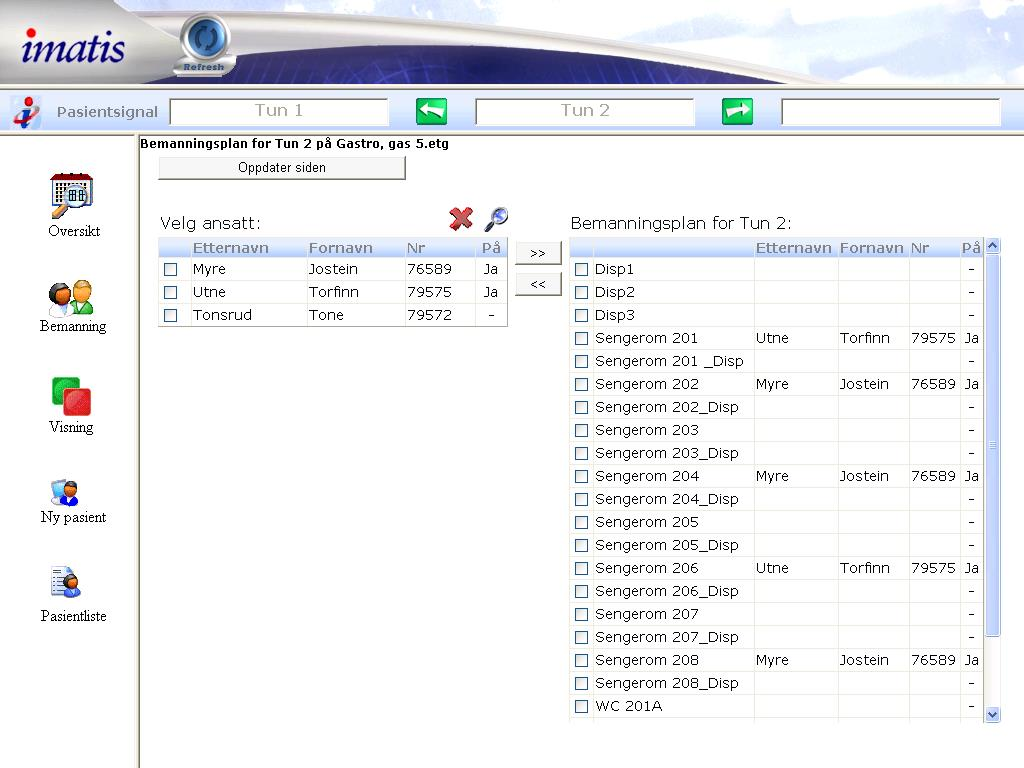
\includegraphics[scale=0.5]{bemanningsplan.jpg}
\caption{Bemanningsplan}
\label{bemanningsplan}
\end{figure}

\noindent
Funksjonen visning, vist i figur \ref{visning}, viser en oversikt over pasientsignalanlegget ved gjeldende sengetun, her vist som Gastro i 5. etasje, tun en og to. Grønn T markerer at pleiepersonell har trykket på den grønne knappen på rompanelet i det gjeldende sengerommet, og tilsynelatende er tilstede. Dette er ikke nødvendigvis riktig, da pleiepersonell kan glemme å trykke av den grønne knappen da de forlater rommet. Rød S signaliserer et pasientsignal, mens innrammet rød H signaliserer et hasteanrop. Rødt kryss varsler feil i systemet.

\begin{figure}[H]
\centering
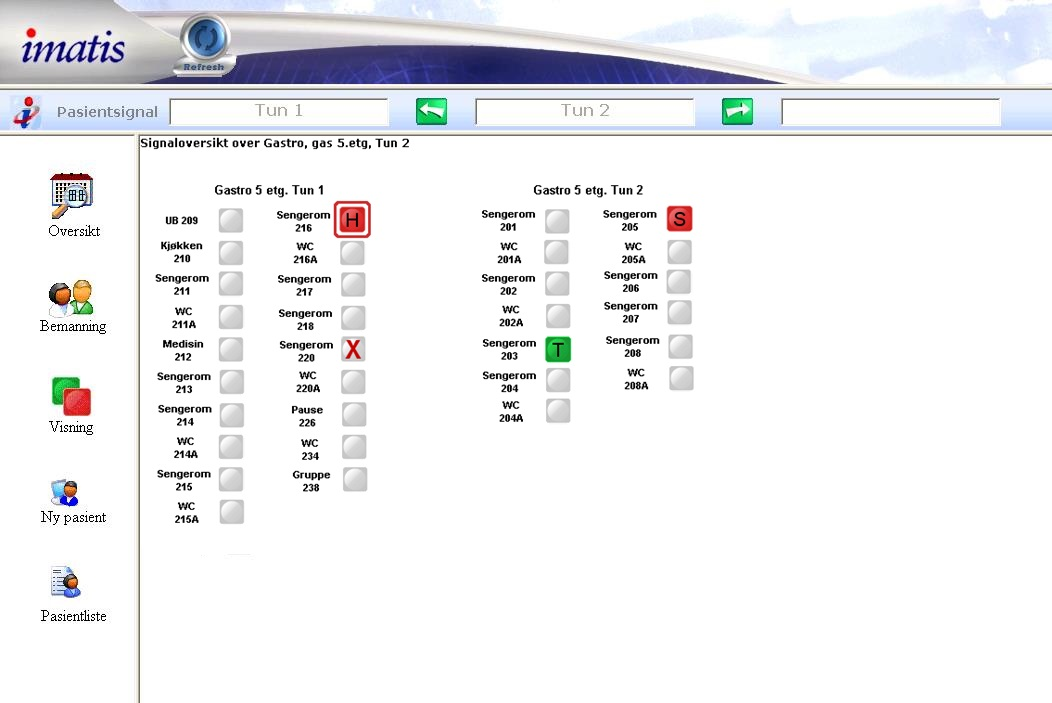
\includegraphics[scale=0.5]{pasientapplikasjon.jpg}
\caption{Visning}
\label{visning}
\end{figure}

\subsubsection{Trådløs telefonenhet}
De trådløse telefonenhetene inngår i det IP-baserte telefonisystemet ved St. Olavs Hospital, og er av typen Cisco Wireless IP Phone 7921G. I tillegg til å tilby basisfunksjoner som å ringe og sende tekstmeldinger, støtter de tjenester for alarmering. Pleiepersonell logger seg på telefonene for å motta pasientsignal og hasteanrop i forhold til ansvar gitt i bemanningsplanen.

\subsubsection{Pasientterminal}
Pasientterminalen inneholder en rekke funksjoner som pasienten kan benytte seg av, deriblant TV, radio, telefon, internett, spill og knapp for pasientsignal. Den røde knappen under skjermen benyttes for å utløse pasientsignal, og denne fungerer uavhengig av om terminalen er skrudd på eller ikke.

\pagebreak

\subsection{Hvordan det hele henger sammen}
\begin{figure}[H]
\centering
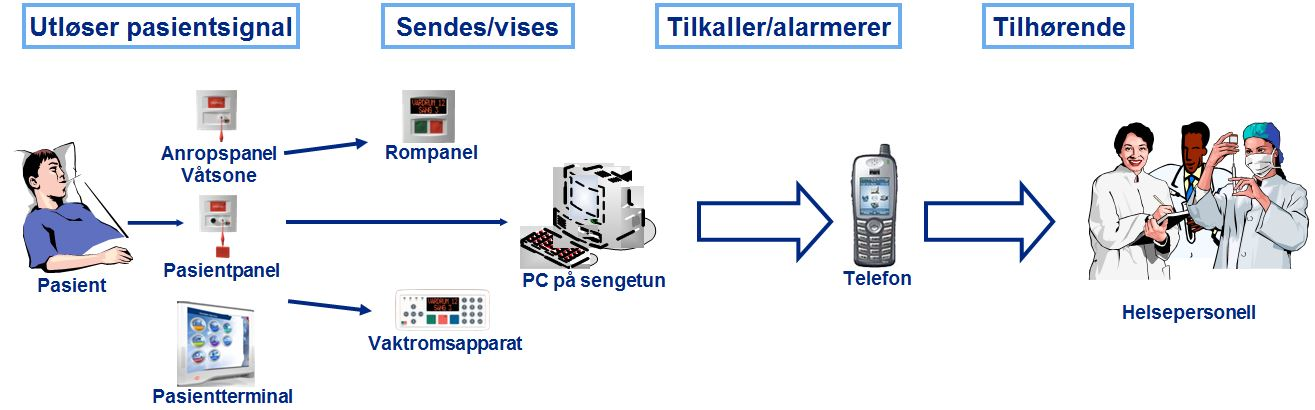
\includegraphics[scale=0.5]{alarmprosess.jpg}
\caption{Pasientsignal (Opplæring:Pasientsignal, delvis modifisert)}
\label{alarmprosess}
\end{figure}

\noindent
Pasienten kan utløse et pasientsignal ved å trykke på signalknappen på pasientterminalen, dra i snoren på anropspanelet, eller trykke på den røde knappen på rompanelet. Da vil lysdioden på rompanelet og anropspanelet blinke rødt. På andre sengerom hvor tilstedemarkering er aktivert vil lysdioden blinke rødt, og nummer- og stedsangivelse vil vises på displayet. Vaktromsapparatet vil blinke og avgi lydsignal, og pasientsignalapplikasjonen viser markering for pasientsignal.

\begin{figure}[H]
        \centering
        \begin{subfigure}[b]{0.35\textwidth}
        		\centering
                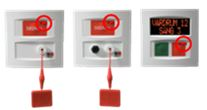
\includegraphics[scale=0.7]{signal_paneler.jpg}
        \end{subfigure}
        \begin{subfigure}[b]{0.35\textwidth}
        		\centering
                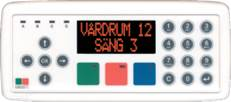
\includegraphics[scale=1]{vaktromsapparat.jpg}
                \label{telefon}
        \end{subfigure}
        \caption{Alarmering ved pasientsignal}\label{pasientsignalalarm}
\end{figure}

\begin{figure}[H]
\centering
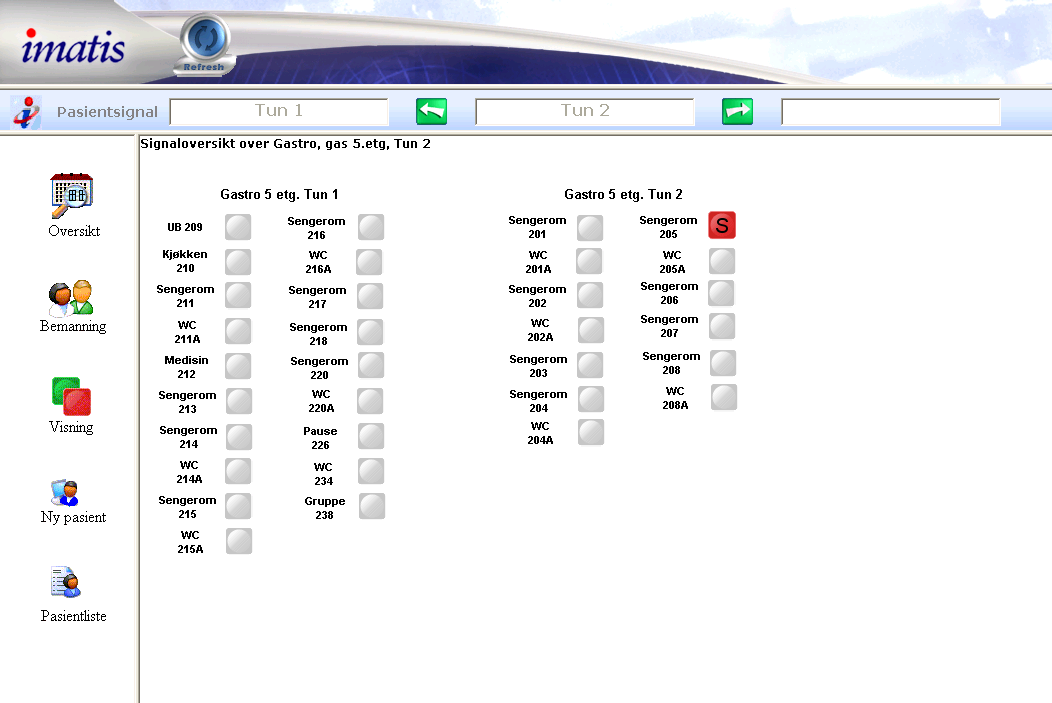
\includegraphics[scale=0.4]{applikasjonalarm.png}
\caption{Pasientsignalapplikasjon ved alarm (Brukermanual for Pasientsignal og Pasientsignalapplikasjon )}
\label{alarmprosess}
\end{figure}

\noindent
Dedikert pleiepersonell registrert i bemanningsplanen tilkalles på sin trådløse telefonenhet ved at melding vises på displayet, og lydsignal avgis. Mottaker har da mulighet til å godta eller avvise pasientsignalet. Dersom vedkommende velger å avvise tilkallingen, eller ikke foretar seg noe innen 15 sekunder, vil signalet sendes videre til neste ressurs. Slik vil det fortsette inntil tilkallingen blir bekreftet.

\begin{figure}[H]
\centering
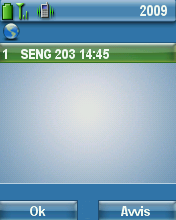
\includegraphics[scale=1]{alarmtelefon.png}
\caption{Trådløs telefonenhet ved alarm (Opplæring: Pasientsignal)}
\label{alarmprosess}
\end{figure}

\noindent
Dersom mottaker godtar tilkallingen vil den legges i mottakers arbeidsliste, og vedkommende har 2 minutter på seg for å tilstedemarkere seg på rommet, ellers vil tilkallingen videresendes til neste registrerte ressurs.

\begin{figure}[H]
\centering
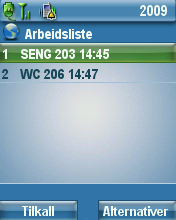
\includegraphics[scale=1]{telefonok.png}
\caption{Arbeidsliste (Opplæring: Pasientsignal)}
\label{alarmprosess}
\end{figure}

\noindent
Ved tilstedemarkering vil lyssignalet stoppe på anropspanelene, og rompanelet vil blinke med grønt lys. Vaktromsapparatet viser sengenummer og stopper lydsignalet, tilkallingen fjernes fra mottakers arbeidsliste, og pasientsignalapplikasjonen viser tilstedemarkering.
 
\begin{figure}[H]
        \centering
        \begin{subfigure}[b]{0.35\textwidth}
        		\centering
                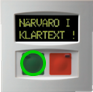
\includegraphics[scale=1]{rompanelok.png}
                \caption{Rompanel}
                \label{rompanelok}
        \end{subfigure}
        \begin{subfigure}[b]{0.25\textwidth}
        		\centering
                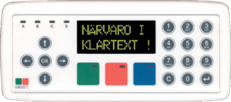
\includegraphics[scale=0.9]{vaok.png}
                \caption{Vaktromsapparat}
                \label{vaok}
        \end{subfigure}
        \caption{Det faste systemet etter tilstedemarkering}
\end{figure} 

\begin{figure}[H]
\centering
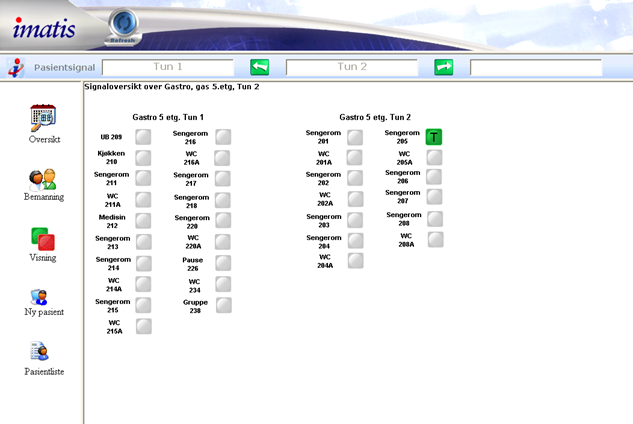
\includegraphics[scale=1]{applikasjonok.png}
\caption{Pasientsignalapplikasjon etter tilstedemarkering}
\label{applikasjonok}
\end{figure}

\noindent
Pleiepersonell trykker på den grønne knappen for å avstille pasientsignalet. Dersom pleiepersonell får behov for assistanse kan han/hun utløse et hasteanrop ved å bruke signalknappen på anropspanelet eller den røde knappen på rompanelet. Alarmen indikeres ved et hastig lydsignal, og røde tall for romnummer og stedsangivelse blinker hurtig på vaktromsapparatet og tilstedemarkerte rompaneler. På det gjeldende rommet vil både rød og grønn lysdiode blinke på rompanelet. I tillegg sendes en hasteanropsmelding, som ikke kan avvises, til samtlige av pleiepersonellets trådløse telefoner på sengetunet. Pasientsignalapplikasjonen viser markering for hasteanrop. Hasteanrop legges i arbeidsliste og avstilles på samme måte som pasientsignaler.

\begin{figure}[H]
\centering
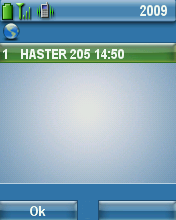
\includegraphics[scale=1]{hasteanropsmelding.png}
\caption{Trådløs telefonenhet ved hasteanrop}

\begin{figure}[H]
\centering
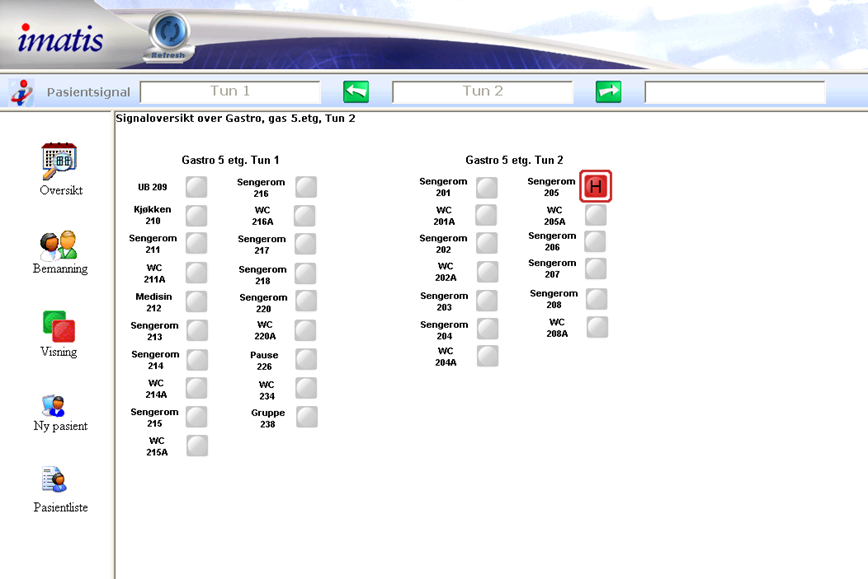
\includegraphics[scale=1]{applikasjonhast.png}
\caption{Pasientsignalapplikasjon ved hasteanrop}
\label{applikasjonok}
\end{figure}
\label{applikasjonok}
\end{figure}











\chapter{Plan for Workshop}
\label{appendix_workshop}


\textbf{Dette gjøres på forhånd:}
\begin{itemize}
  \item Klargjøre laben og artefakter
  \item Lage navneskilt
\end{itemize}

%\begin{adjustbox}{with=\textwith, hight=\texthight}
\begin{table}[H]
%\small
\caption{Overordnet plan for dagen}
%\centering
\begin{tabular}{l|l|l|l|l}
\hline
\textbf{\begin{tabular}[x]{@{}c@{}}Del av\\workshop\end{tabular}} & \textbf{Beskrivelse} & \textbf{Hvor} & \textbf{Tidspunkt} & \textbf{Varighet}\\
\hline
Steg 1 & Informasjon & \begin{tabular}[x]{@{}c@{}}Rundt bord\\/i gangen\end{tabular} & 13:00-13:15 & 15min\\
\hline
Steg 2 & Fokusgruppe med scenarier & \begin{tabular}[x]{@{}c@{}}Rundt bord\\/i gangen\end{tabular} & 13:15-13:45 & 30min\\
\hline
& \textbf{Pause} & & 13:45-13.50 & 5min\\
\hline
Steg 3 &\begin{tabular}[x]{@{}c@{}} Scenarioer med rollespill\\- uten prototype\end{tabular} & Inne på sengerom & 13:50-14:25 & 35min\\
\hline
& \begin{tabular}[x]{@{}c@{}}Scenarioer med rollespill\\- med prototype\end{tabular} & Inne på sengerom & 14:25-15:00 & 35min\\
\hline
& \textbf{Pause} & & 15:00-15:15 & 15min\\
\hline
Steg 4 & Fokusgruppe/oppsummering & \begin{tabular}[x]{@{}c@{}}Rundt bord\\/i gangen\end{tabular} & 15:15-16:00 & 45min
\end{tabular}
\label{OverordnetPlan}
\end{table}
%\end{adjustbox}

\pagebreak

\textbf{Forskningsspørsmål:}
\begin{enumerate}
  \item Identifisere behov knyttet til funksjonalitet for støtte av distribusjon av awareness-informasjon.
  \item Hvordan kan systemet endres for å begrense potensielle negative effekter ved avbrytelser?
\end{enumerate}

\subsubsection{Steg1: Informasjon - 13:00-13:15 (15min)}
\begin{itemize}
  \item Ønsker velkommen
  \item Presentasjonsrunde
  \item Presentasjon av roller (fasilitator, pasienter etc\ldots)
  \item Presenterer planen for workshopen og dens hensikt
  \begin{itemize}
  \item Vil vil først ha en felles diskusjon her, hvor vi ønsker å avdekke dagens situasjon mtp ansvarsfordeling og organisering av arbeidet
  	\item Vi vil deretter spille ut et par scenarioer på sengerommene her, hvor dere bruker de telefonene og funksjonene dere er vant med
  	\item Deretter vil vi forklare funksjonaliteten til prototypen vi har laget, for så å spille ut et par scenarier hvor vi ønsker at dere skal bruke denne
  	\item Til sist ønsker vi en oppsumering/diskusjon rundt disse scenarioene og deres syn på prototypen
  \end{itemize}
\end{itemize}

\noindent
Vi ønsker at alle bidrar i alle diskusjonene. Vi er her fordi vi ønsker å høre deres tanker/meninger

\subsubsection{Steg 2: Fokusgruppe med scenarioer}

\begin{table}[H]
\small
\caption{Scenarioer til fokusgruppe}
\begin{tabular}{p{4cm}|p{5cm}|l|l}
\hline
\textbf{Scenario} & \textbf{Oppfølgingsspørsmål} & \textbf{Tidspunkt} & \textbf{Varighet}\\
\hline
\emph{Rollen som primærsykepleier:} Du har ansvar for to av pasientene på tunet. \textbf{Hvordan vil du definere/beskrive denne rollen?} & I hvilken grad kjenner du til de andre pasientene? \begin{itemize}
\item Hvem har ansvar?
\item sykdomsbilde og tilstand
\item lokasjon
\item hvem og hvilket type rom
\end{itemize}
& 13:15-13:25 & 10min\\
\hline
\emph{Rollen som disp:} Du er disp for to av pasientene på tunet. \textbf{Hvordan vil du definere/beskrive denne rollen?} & I hvilken grad påvirker det beslutningen du tar om å svare på et pasientsignal, når du får et anrop fra en pasient du er disp for?
 & 13:25-13:35 & 10min\\
\hline
\emph{Utilgjengelig:} Du havner i en situasjon hvor du vil være utilgjengelig i en periode.
\begin{itemize}
\item i hvilke situasjoner er det ønskelig å kunne være “utilgjengelig” for henvendelser?
\item Hvilke henvendelser vil du ønske å motta uansett situasjon?
\item Hvilke henvendelser vil du helst ikke motta? Hvorfor?
\end{itemize}
& 
\begin{itemize}
\item Hvem informeres (kolleger/pasienter)?
\item Hva med telefonen?
\item Endres bemanningsplanen?
\item Lunchpause?
\item sårskift?
\item Urolig psient?
\item Andre situasjoner?
\end{itemize}
& 13:35-13.45 & 10min\\
\end{tabular}
\label{Steg2}
\end{table}

\textbf{Pause - 5min}
\pagebreak
\subsubsection{Steg 3: Scenarioer med rollespill}



\begin{itemize}
\item Presentasjon av pasientenes sykdomshistorier rundt bordet før vi starter rollespillene
\end{itemize}

\begin{table}[H]
\small
\caption{Scenario 1 for pasientsignal uten prototype}
\begin{tabular}{p{3cm}|p{2cm}|p{4cm}|l|l}
\hline
\textbf{Scenario} & \textbf{Aksjon} & \textbf{Oppfølgingsspørsmål} & \textbf{Tidspunkt} & \textbf{Varighet}\\
\hline
Du står i gangen, en annen sykepleier er også til stede. Du skal inn til Jonas fordi du vet han er veldig usikker og bekymret, og vil høre hvordan det går & & Hva slags forberedelser gjør du og hvorfor? (sier du fra til andre?)
& 13:50-13:55 & 5min\\
\hline
Du er inne hos Jonas og har en seriøs samtale om hans tilstand & Adam utløser pasientsignal. & 
\begin{itemize}
\item Hva gjør du?
\item Hvor ser du?
\item Ønsker du å fortsette samtalen uavbrutt eller forlater du rommet?
\item Hvordan påvirker signalet situasjonen?
\item Hvilken informasjon ville satt deg i bedre stand til å ta en avgjørelse?
\item Hvis du ikke velger å forlate rommet, hvorfor blir du?
\item Dersom du forlater rommet, og det viser seg at Adam ønsket et glass vann, føler du at du tok riktig avgjørelse?
\end{itemize}
 & 13:55-14:00 & 5min\\
\end{tabular}
\label{Steg3.1}
\end{table}

\begin{table}[H]
\small
\caption{Scenario 2 for pasientsignal uten prototype}
\begin{tabular}{p{3cm}|p{2cm}|p{4cm}|l|l}
\hline
\textbf{Scenario} & \textbf{Aksjon} & \textbf{Oppfølgingsspørsmål} & \textbf{Tidspunkt} & \textbf{Varighet}\\
\hline
Du står i gangen, en annen sykepleier er også til stede. Du skal inn til Adam for å utføre sårskift, og har kledd deg opp med stellefrakk  mm. & & Hva slags forberedelser gjør du og hvorfor? (sier du fra til andre?)
& 14:05-14:10 & 5min\\
\hline
Du er inne hos Adam og Utfører sårskift & Jonas utløser pasientsignal. & 
\begin{itemize}
\item Hva gjør du?
\item Hvor ser du?
\item Ønsker du å fortsette sårskiftet eller forlater du rommet? Hvilke faktorer spiller inn?
\item Hvordan påvirker signalet situasjonen?
\item Hvordan blir arbeidet påvirket?
\item Ville du satt deg som utilgjengelig? Sagt fra til noen om at du skal foreta et sårskift?
\item Dersom du forlater rommet, og det viser seg at Jonas ønsket et glass vann, føler du at du tok riktig avgjørelse?
\end{itemize}
 & 14:10-14:25 & 15min\\
\end{tabular}
\label{Steg3.2}
\end{table}

\pagebreak

\begin{table}[H]
\small
\caption{Scenario 1 for pasientsignal med prototype}
\begin{tabular}{p{3cm}|p{2cm}|p{4cm}|l|l}
\hline
\textbf{Scenario} & \textbf{Aksjon} & \textbf{Oppfølgingsspørsmål} & \textbf{Tidspunkt} & \textbf{Varighet}\\
\hline
Du er inne hos Jonas og har en seriøs samtale om hans tilstand & Adam utløser pasientsignal & \begin{itemize}
\item Hva gjør du?
\item Hvor ser du?
\item Ønsker du å fortsette samtalen uavbrutt eller forlater du rommet? Hvilke faktorer spiller inn?
\item Hvordan påvirker signalet situasjonen?
\item Hvordan blir arbeidet påvirket?
\item Hvis du ikke velger å forlate rommet, hvorfor blir du?
\item Dersom du forlater rommet, og det viser seg at Adam ønsket et glass vann, føler du at du tok riktig avgjørelse?
\item Ville du brukt “kontakter” for å se de andre sin status
\item Om du merker at Jonas trenger at du er der en stund, ville du satt deg som opptatt? (rød)
\item Kommentarer til design?
\end{itemize}
& 14:25-14:40 & 15min\\
\end{tabular}
\label{Steg3.3}
\end{table}

\begin{table}[H]
\small
\caption{Scenario 2 for pasientsignal med prototype}
\begin{tabular}{p{3cm}|p{2cm}|p{4cm}|l|l}
\hline
\textbf{Scenario} & \textbf{Aksjon} & \textbf{Oppfølgingsspørsmål} & \textbf{Tidspunkt} & \textbf{Varighet}\\
\hline
Du er inne hos Adam og utfører sårskift. & Jonas utløser pasientsignal. \emph{Telefonen vibrerer} & \begin{itemize}
\item Hva gjør du?
\item Hvor ser du?
\item Ønsker du å fortsette sårskiftet eller forlater du rommet? Hvilke faktorer spiller inn?
\item Hvordan påvirker signalet situasjonen?
\item Hvordan blir arbeidet påvirket?
\item Hvis du ikke velger å forlate rommet, hvorfor blir du?
\item Ville du satt deg som utilgjengelig? Sagt fra til noen om at du skal foreta et sårskift?
\item Ville du brukt “kontakter” for å se de andre sin status
\item Kommentarer til design?
\end{itemize}
& 14:40-15:00 & 20min\\
\end{tabular}
\label{Steg3.4}
\end{table}

\textbf{Pause - 15min}

\pagebreak

\subsubsection{Steg 4: Fokusgruppe/Sammendrag - 15:15-16:00 (45min)}

\begin{itemize}
\item Oppsummering av scenarioene
	\begin{itemize}
	\item Var situasjonene som ble utspilt relevante? Eventuelt hvorfor ikke?
\item Forslag til oppfølgingsspørsmål:
	\item Tror dere noe av den løsningen vi foreslo kan være av nytte?
	\item Kan dere se for dere noe sånt i bruk?
	\item I forhold til å ta avgjørelsen om dere skal forlate pasienten til fordel for pasienten som ringer - synes dere prototypen ga tilstrekkelig informasjon?
		\item Er det annen informasjon dere kunne tenke dere?
	\item Tror dere informasjonen prototypen gir vil gjøre avbrytelsene mindre forstyrrende?
	\item Tror dere funksjonen om tilstedeværelsen til andre sykepleiere vil gjøre avbrytelsene mindre forstyrrende?
	\end{itemize}
\end{itemize}

\end{document} 
